\documentclass[12pt]{article}
\usepackage[latin1]{inputenc}
\usepackage[T1]{fontenc}
\usepackage{palatino}
\usepackage{fancyheadings}
\usepackage{float}
\usepackage{subfigure}
\usepackage{wrapfig}
\usepackage[dvips]{graphics}
\usepackage{graphicx}
\usepackage{epsfig}
\usepackage{multicol}
\usepackage{color}
\usepackage{url}
\usepackage{html}

\setlength{\topmargin}{0cm}
\setlength{\headheight}{1cm}
\setlength{\textheight}{21cm}
\setlength{\textwidth}{16cm}
\setlength{\oddsidemargin}{0cm}
\setlength{\evensidemargin}{0cm}
\setlength{\columnsep}{0.125in}
\setlength{\columnseprule}{0.5pt}
\setlength{\footskip}{1cm}
\sloppy

\newcommand{\image}[4]
%	   {\begin{figure}[htbp]
	   {\begin{figure}[h!]
            \includegraphics[width=#2\textwidth]{#1}
	    \end{figure}
	   }
% \image{fig.eps}{scale}

%--------------------------------- page style --------------------------------
\pagestyle{fancy}
\rhead{}
\lhead{}
\rfoot{\thepage}
\lfoot{}
\cfoot{}
%---------------------------------- document ---------------------------------
\date   {}
\title  {Stratus User's Manual}
\author {Sophie Belloeil}

\begin{document}

\setlength{\footrulewidth}{0.6pt}
\maketitle

%%\begin{htmlonly}
%%  \htmlrule
%%  \noindent La version imprimable de ce document est disponible ici~: \\
%%  \begin{center}
%%    \hyperref[hyper]{http://asim.lip6.fr/~jpc/M1-C++/TME/6/TME6.pdf}{}{}
%%                    {http://asim.lip6.fr/~jpc/M1-C++/TME/6/TME6.pdf}
%%  \end{center}
%%\end{htmlonly}

\tableofchildlinks
\htmlrule

\section{Introduction}
\label{secintroduction}

    \subsection{Stratus}
    \label{secstratus}
    \subsubsection{Name}

Stratus -- Procedural design language based upon \emph{Python}

\subsubsection{Description}

\emph{Stratus} is a set of \emph{Python} methods/functions dedicated to procedural generation purposes. From a user point of view, \emph{Stratus} is a circuit's description  language that allows \emph{Python} programming flow control, variable use, and specialized functions in order to handle vlsi objects.\\

\indent Based upon the \emph{Hurricane} data structures, the \emph{Stratus} language gives the user the ability to describe netlist and layout views.

\subsubsection{Creation of a cell}

A cell is a hierachical structural description of a circuit in terms of ports (I/Os), signals (nets) and instances :

\begin{itemize}
\item Method \verb-Interface-
    \begin{itemize}
        \item LogicIn
        \item LogicOut
        \item LogicInOut
        \item TriState
        \item VddIn
        \item VssIn
    \end{itemize}
\item Method \verb-Netlist-
    \begin{itemize}
        \item Signal
        \item Inst
        \item Facilities : \&, |, +, Mux, Shift, Eq/Ne ...
    \end{itemize}
\item Method \verb-Layout-
    \begin{itemize}
        \item Place, PlaceTop, PlaceBottom, PlaceRight, PlaceLeft
        \item SetRefIns
        \item DefAb, ResizeAb
        \item PlaceCentric
        \item PlaceGlue, FillCell
        \item PadNorth, PadSouth, PadEast, PadWest
        \item AlimVerticalRail, AlimHorizontalRail
        \item AlimConnectors
        \item PowerRing
        \item RouteCk
    \end{itemize}
    \item Method \verb-Pattern-
    \item Method \verb-View-
    \item Method \verb-Save-
\end{itemize}

\subsubsection{Syntax highlighting}

This chapter describes what to do to have the right syntax highlighting when using vi.

\begin{itemize}
    \item Commands to do when you want to change once the coloration of your file :
\end{itemize}
\begin{small}
\begin{verbatim}
:syntax off
:source /asim/coriolis/share/etc/stratus.vim
\end{verbatim}
\end{small}
\begin{itemize}
    \item Modification of your .vimrc in order to have the syntax highlighting each time you open a file :
\end{itemize}
\begin{small}
\begin{verbatim}
syntax off
autocmd BufRead,BufNewfile *.py so /asim/coriolis/share/etc/stratus.vim
syntax on
\end{verbatim}
\end{small}
        
\subsubsection{Environment variables}

\begin{itemize}
    \item CRL\_IN\_LO, default value : \verb-def-
    \item CRL\_OUT\_LO, default value : \verb-def-
    \item CRL\_IN\_PH, default value : \verb-def-
    \item CRL\_OUT\_PH, default value : \verb-def-
    \item CRL\_CATA\_LIB, default value : \verb-.-
    \item CRL\_CATAL\_NAME, default value : \verb-CATAL-
\end{itemize}

\subsubsection{Syntax}

A \emph{Stratus} file must have a .py extension and must begin as follow :
\begin{verbatim}
#!/usr/bin/python

from stratus import *
\end{verbatim}

\indent In order to execute a \emph{Stratus} file (named \verb-file- for example), one has two choices :
\begin{verbatim}
python file.py
\end{verbatim}
\indent Or :
\begin{verbatim}
chmod u+x file.py
./file.py
\end{verbatim}

\indent The names used in \emph{Stratus}, as arguments to \emph{Stratus} functions, should be alphanumerical, including the underscore. The arguments of \emph{Stratus} are case sensitive, so \textsc{VDD} is not equivalent to \textsc{vdd}.\\
    
\indent Vectorized connectors or signal can be used using the \textsc{[n:m]} construct.\\

\subsubsection{Example}

You can see a concrete example at : \hyperref[ref]{\emph{A concrete example}}{}{Example}{secexample}

\subsubsection{See Also}

\hyperref[ref]{\emph{Model}}{}{Model}{secmodel}
\hyperref[ref]{\emph{Param}}{}{Param}{secparam}
\hyperref[ref]{\emph{Example}}{}{Example}{secexample}
\hyperref[ref]{\emph{Netlist}}{}{Netlist}{secnetlist}
\hyperref[ref]{\emph{Layout}}{}{Layout}{seclayout}
\hyperref[ref]{\emph{Place and Route}}{}{Place and Route}{secroute}
\hyperref[ref]{\emph{Facilities}}{}{Facilities}{secfacilities}

    \subsection{Class Model}
    \label{secmodel}
    \subsubsection{Name}

Model -- Master class

\subsubsection{Description}

Every cell made is a class herited from class \verb-Model-.\\
\indent Some methods have to be created, like \verb-Interface-, \verb-Netlist- ... Some methods are inherited from the class \verb-Model-.

\subsubsection{Parameters}

\begin{itemize}
    \item \verb-name- : The name of the cell (which is the name of the files which will be created)
    \item \verb-param- : A dictionnary which gives all the parameters usefull in order to create the cell
\end{itemize}
  
\subsubsection{Methods}

Methods of class \verb-Model- are listed below :
\begin{itemize}
    \item \verb-View- : Opens/Refreshes the editor in order to see the created layout
    \item \verb-Quit- : Finishes a cell without saving
    \item \verb-Save- : Saves the created cell\\If several cells have been created, they are all going to be saved in separated files\\
\end{itemize}

Some of those methods have to be defined in order to create a new cell :
\begin{itemize}
    \item \verb-Interface- : Description of the external ports of the cell
    \item \verb-Netlist- : Description of the netlist of the cell
    \item \verb-Layout- : Description of the layout of the cell
    \item \verb-Vbe- : Description of the behavior of the cell
    \item \verb-Pattern- : Description of the patterns in order to test the cell
\end{itemize} 
    
\subsubsection{Example}

You can see a concrete example at : \hyperref[ref]{\emph{A concrete example}}{}{Example}{secexample}
   
\subsubsection{See Also}

\hyperref[ref]{\emph{Stratus}}{}{Stratus}{secstratus}
\hyperref[ref]{\emph{Param}}{}{Param}{secparam}
\hyperref[ref]{\emph{Example}}{}{Example}{secexample}
\hyperref[ref]{\emph{Netlist}}{}{Netlist}{secnetlist}
\hyperref[ref]{\emph{Layout}}{}{Layout}{seclayout}
\hyperref[ref]{\emph{Place and Route}}{}{Place and Route}{secroute}
\hyperref[ref]{\emph{Facilities}}{}{Facilities}{secfacilities}

    \subsection{Function Param}
    \label{secparam}
    \subsubsection{Name}

Param -- How to use parameters

\subsubsection{Synopsys}

\begin{verbatim}
nbit, nword = Param ( "n", "w" )
\end{verbatim}

\subsubsection{Description}

This function allows the user to give parameters when creating a cell.

\subsubsection{Parameters}

\begin{itemize}
    \item \verb-args- : letters which correspond to letter typed on the shell
\end{itemize}
    
\subsubsection{Example}

When one wants to give values to two parameters, one can type on the shell :
\begin{verbatim}
python test.py -n 4 -w 8
\end{verbatim}

The file \verb-test.py- has then to contain :
\begin{verbatim}
nbit, nword = Param ( "n", "w" )
\end{verbatim}

You can see a concrete example at : \hyperref[ref]{\emph{A concrete example}}{}{Example}{secexample}
    
\subsubsection{Errors}
    
Some errors may occur :
\begin{itemize}
    \item \verb-Error in Param : there is no parameter.-\\The parameters seem to have been forgotten.
\end{itemize}

\subsubsection{See Also}

\hyperref[ref]{\emph{Stratus}}{}{Stratus}{secstratus}
\hyperref[ref]{\emph{Model}}{}{Model}{secmodel}
\hyperref[ref]{\emph{Example}}{}{Example}{secexample}
\hyperref[ref]{\emph{Netlist}}{}{Netlist}{secnetlist}
\hyperref[ref]{\emph{Layout}}{}{Layout}{seclayout}
\hyperref[ref]{\emph{Place and Route}}{}{Place and Route}{secroute}
\hyperref[ref]{\emph{Facilities}}{}{Facilities}{secfacilities}

    \subsection{A concrete example}
    \label{secexample}
    \subsubsection{Addaccu circuit}

\begin{figure}[h!]
\centering
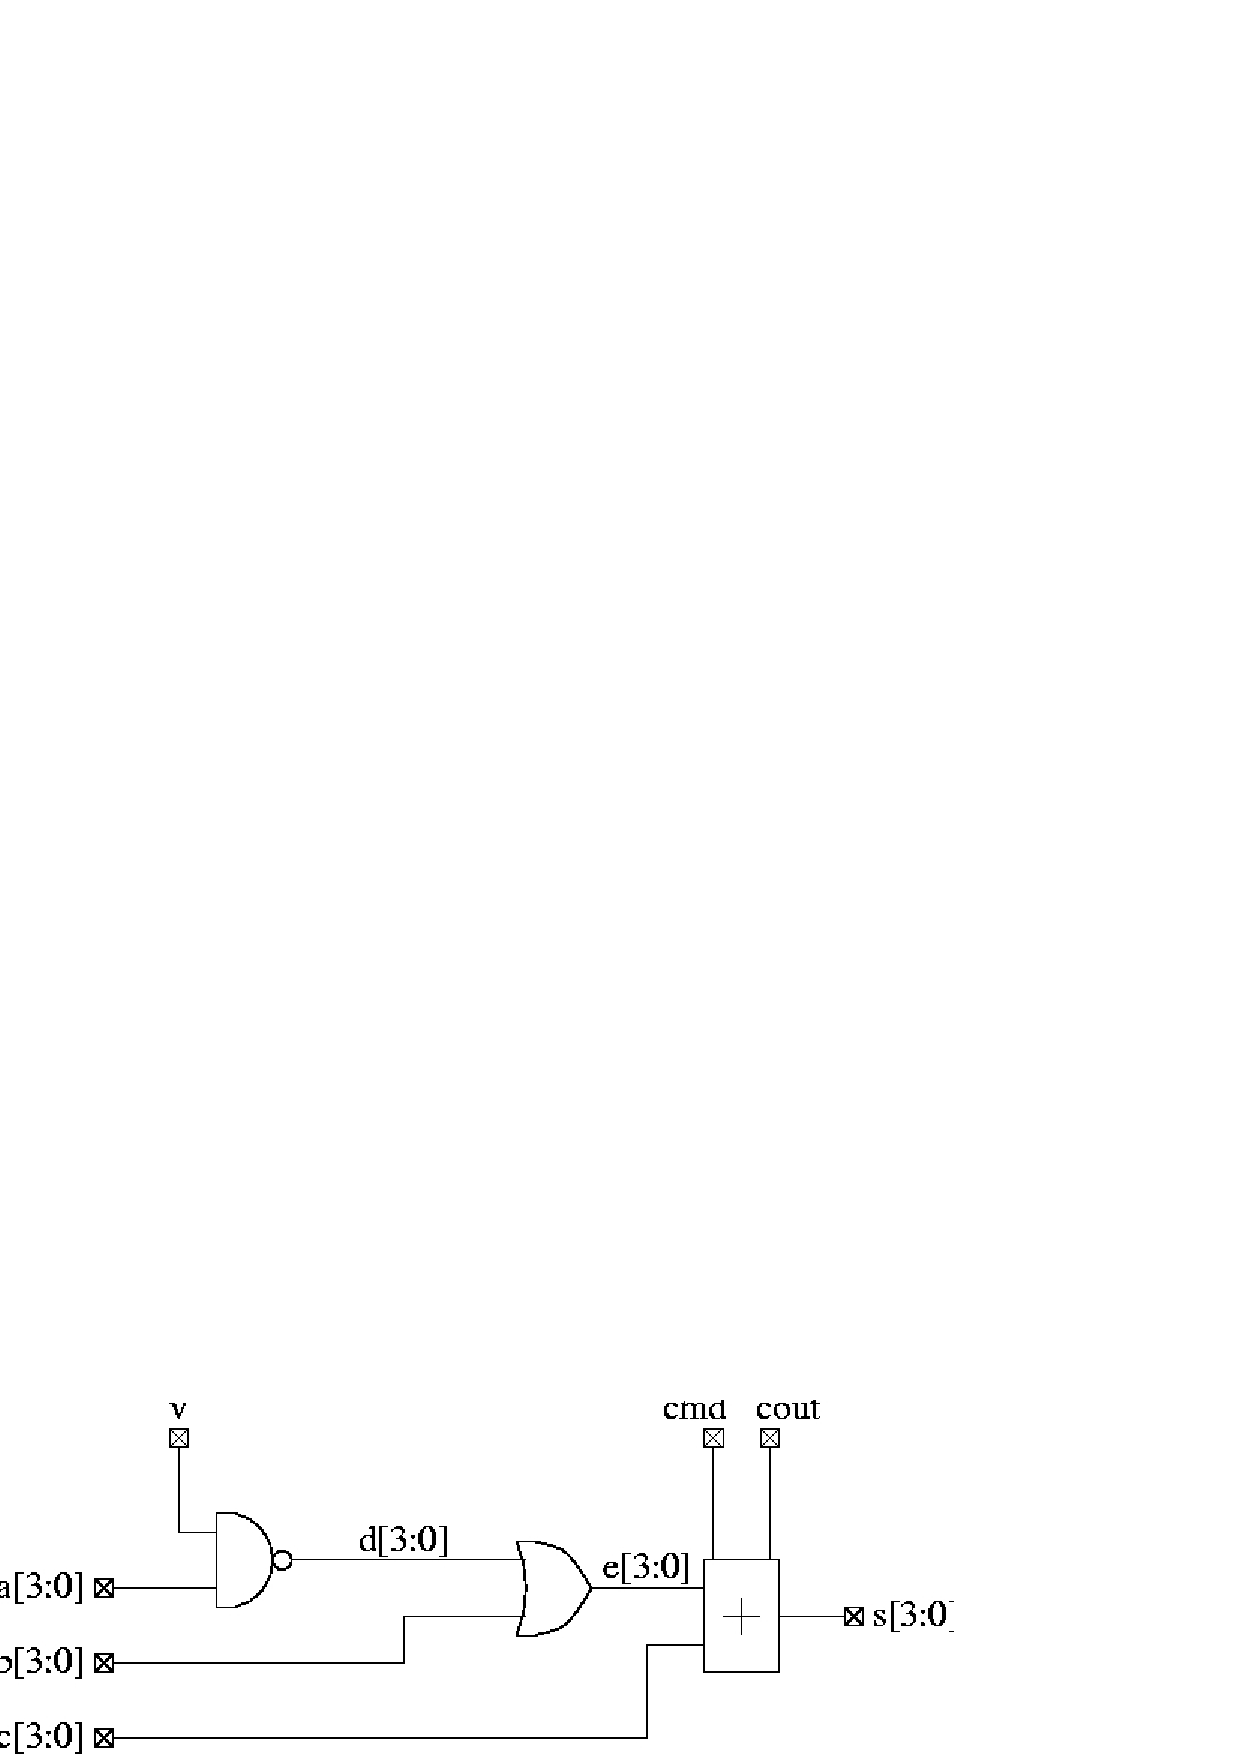
\includegraphics[width=.9\textwidth]{images/add1.png}
\end{figure}
  
\newpage

\subsubsection{Data-path}

\begin{figure}[h!]
\centering
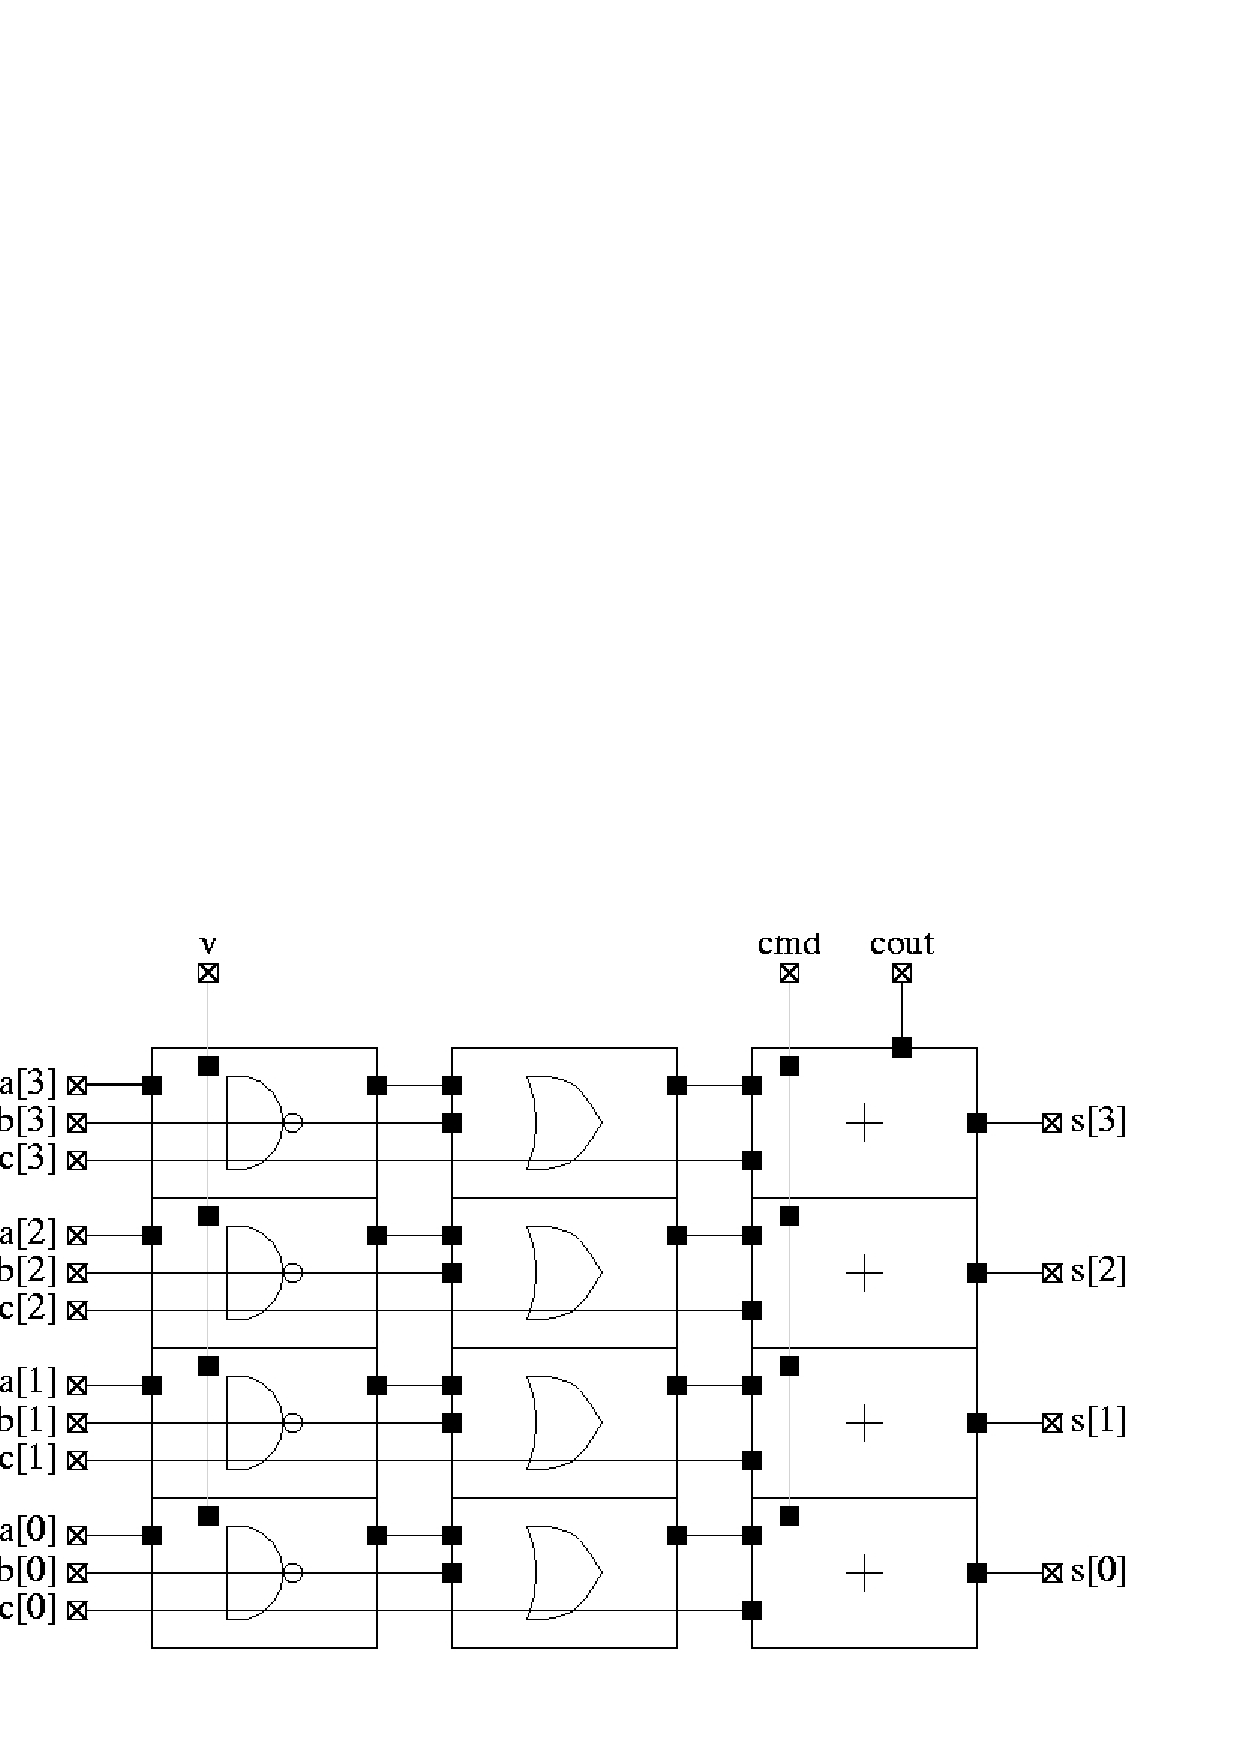
\includegraphics[width=.9\textwidth]{images/add2.png}
\end{figure}

\subsubsection{Description of the circuit with \emph{Stratus}}

\begin{figure}[hbp]
\centering
\includegraphics[width=1.2\textwidth]{images/addaccu.png}
\end{figure}

\newpage

\subsubsection{Creation of the circuit}

\begin{figure}[hbp]
\centering
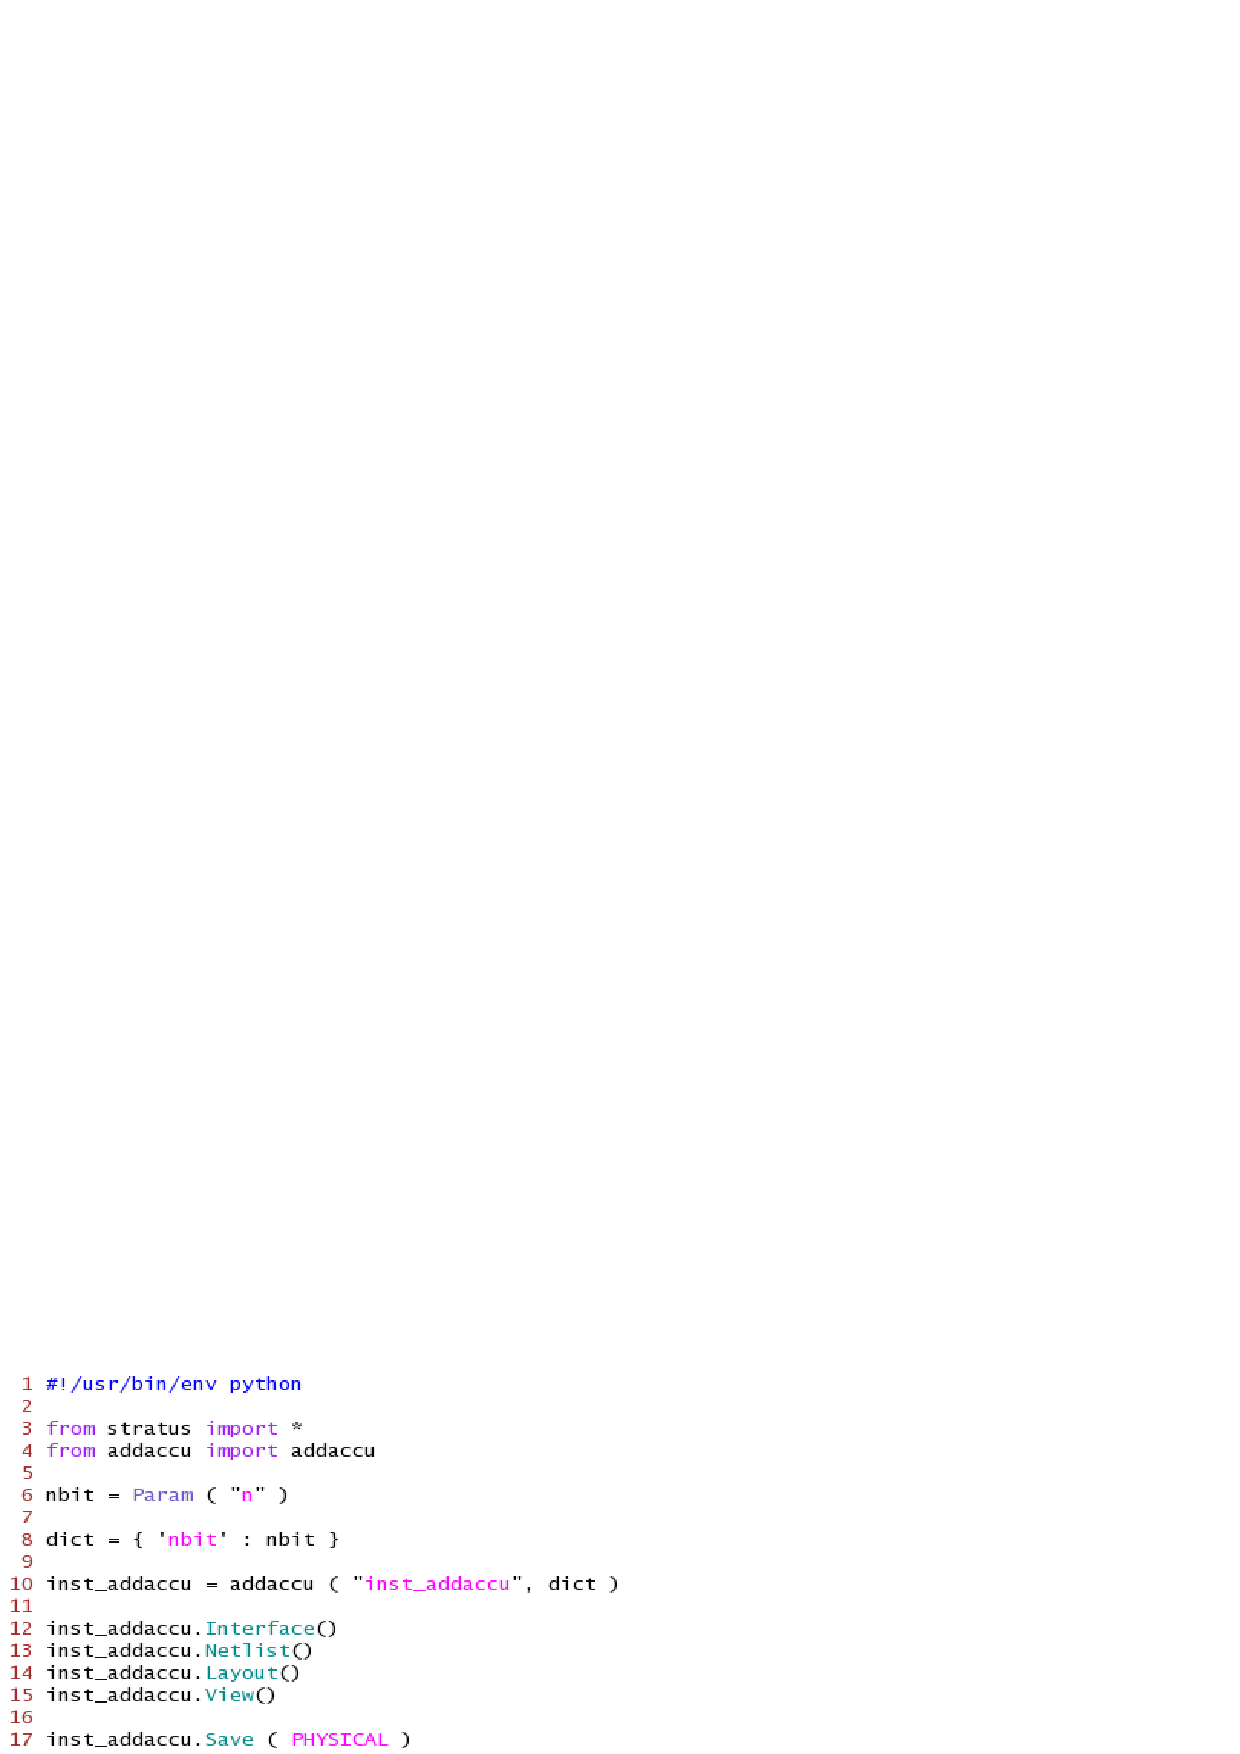
\includegraphics[width=1.3\textwidth]{images/test.png}
\end{figure}

%\newpage
  
\subsubsection{How to execute the file}

\begin{verbatim}
python test.py -n 4
\end{verbatim}
\indent or :
\begin{verbatim}
chmod u+x test.py
./test -n 4
\end{verbatim}

\subsubsection{The editor}

The method \verb-View- permits to open an editor in which one can see the cell being created as shown in the picture below.
\begin{figure}[hbp]
\centering
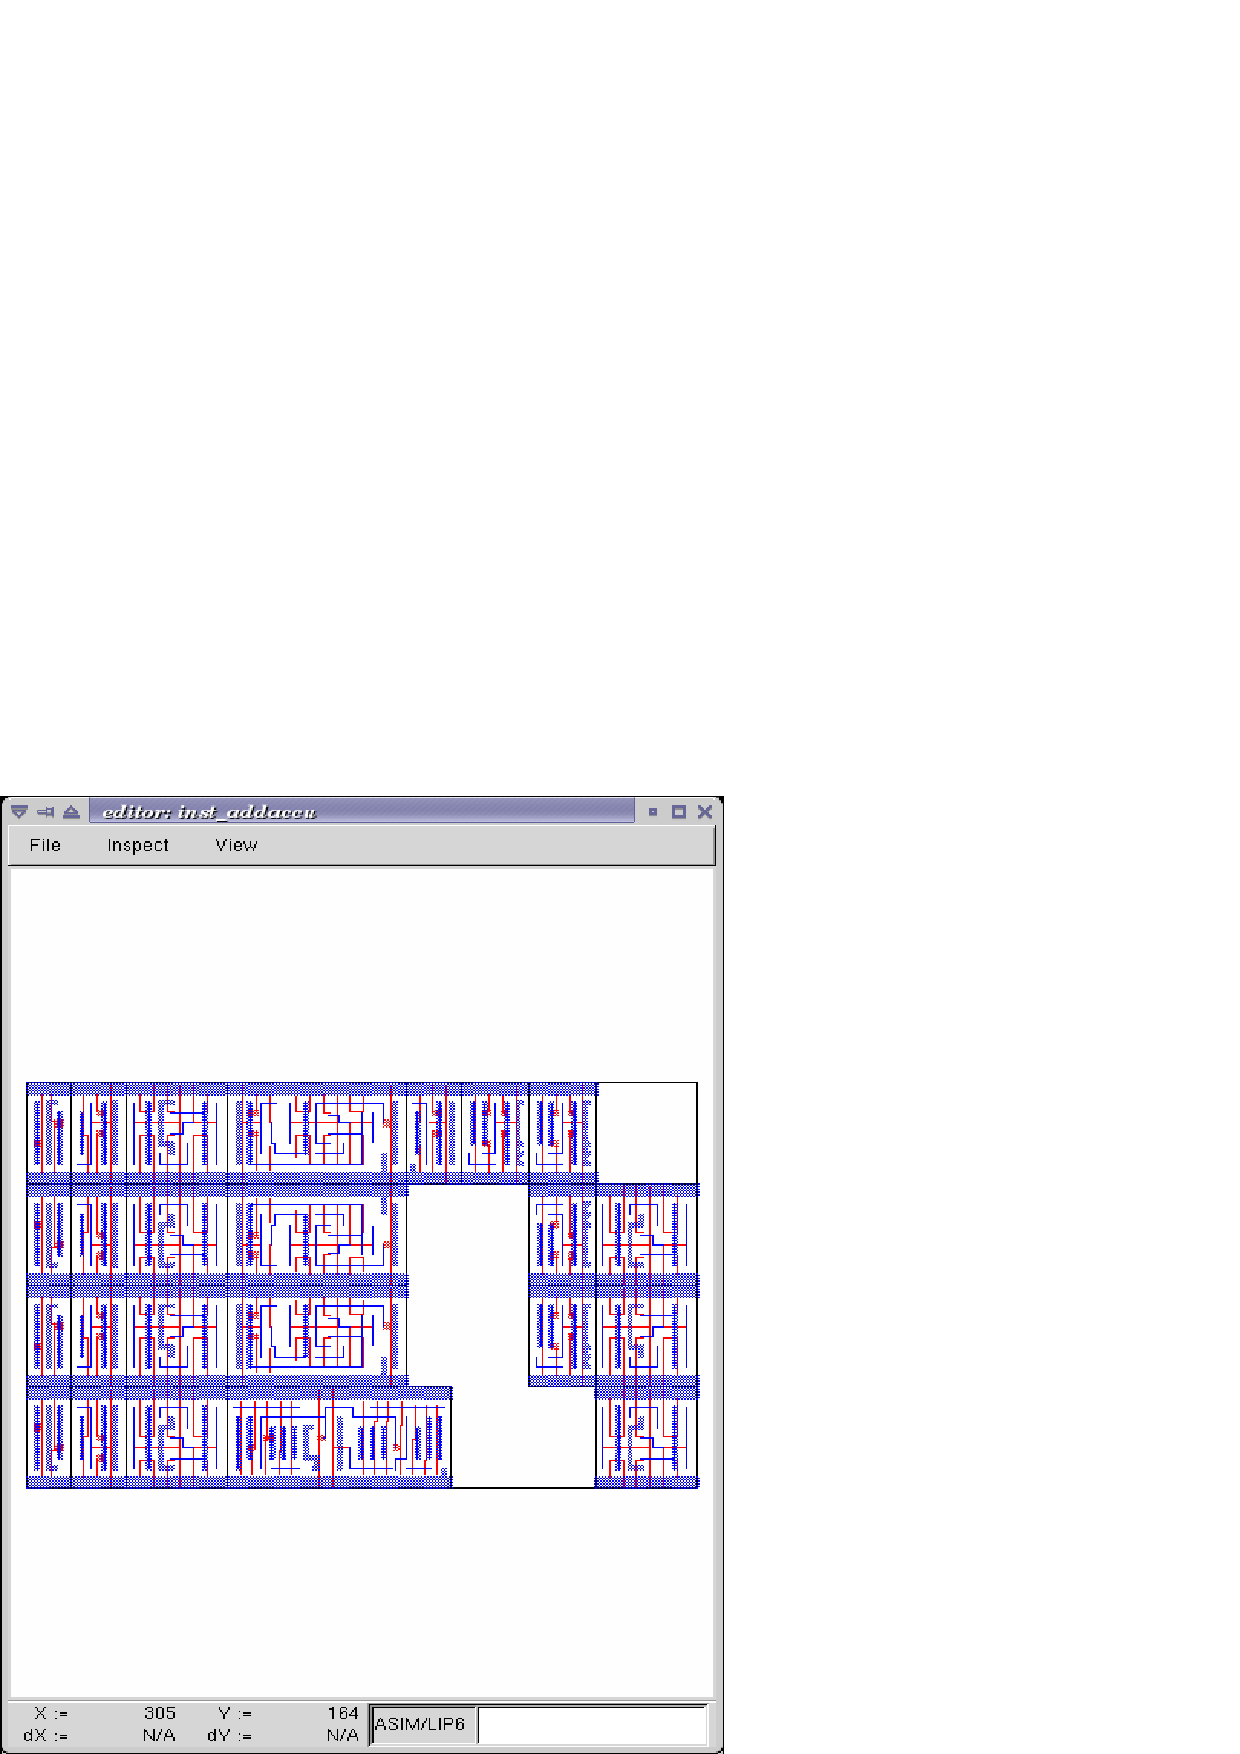
\includegraphics[width=1\textwidth]{images/editor.png}
\end{figure}


\subsubsection{See Also}

\hyperref[ref]{\emph{Stratus}}{}{Stratus}{secstratus}
\hyperref[ref]{\emph{Model}}{}{Model}{secmodel}
\hyperref[ref]{\emph{Param}}{}{Param}{secparam}
\hyperref[ref]{\emph{Netlist}}{}{Netlist}{secnetlist}
\hyperref[ref]{\emph{Layout}}{}{Layout}{seclayout}
\hyperref[ref]{\emph{Place and Route}}{}{Place and Route}{secroute}
\hyperref[ref]{\emph{Facilities}}{}{Facilities}{secfacilities}

   
\newpage 
\section{Description of a netlist}
\label{secnetlist}
    
    \subsection{Creation of nets}
    \label{secnet}
    \subsection{Synopsys}

\begin{verbatim}
netInput = LogicIn ( name, arity )
\end{verbatim}

\subsection{Description}

Instanciation of net. Differents kind of nets are listed below :
\begin{itemize}
    \item \verb-LogicIn- : Creation of an input port
    \item \verb-LogicOut- : Creation of an output port
    \item \verb-LogicInOut- : Creation of an inout port
    \item \verb-LogicUnknown- : Creation of an input/output port which direction is not defined
    \item \verb-TriState- : Creation of a tristate port
    \item \verb-CkIn- : Creation of a clock port
    \item \verb-VddIn- : Creation of the vdd alimentation
    \item \verb-VssIn- : Creation of the vss alimentation
    \item \verb-Signal- : Creation of an internal net
\end{itemize}
        
\subsection{Parameters}

\begin{itemize}
    \item \verb-name- : Name of the net (mandatory argument)
    \item \verb-arity- : Arity of the net (mandatory argument)
    \item \verb-indice- : For buses only : the LSB bit (optional argument : set to 0 by default)\\
\end{itemize}

\indent Only \verb-CkIn, -\verb-VddIn- and \verb-VssIn- do not have the same parameters : there is only the \verb-name- parameter (they are 1 bit nets).

\subsection{Attributes}

\begin{itemize}
    \item \verb-_name- : Name of the net
    \item \verb-_arity- : Arity of the net (by default set to 0)
    \item \verb-_ind- : LSB of the net
    \item \verb-_ext- : Tells if the net is external or not (True/False)
    \item \verb-_direct- : If the net is external, tells the direction ("IN", "OUT", "INOUT", "TRISTATE", "UNKNOWN")
    \item \verb-_h_type- : If the net is an alimentation or a clock, tells the type ("POWER", "GROUND", "CLOCK")
    \item \verb-_type- : The arithmetic type of the net ( "nr" )
    \item \verb-_st_cell- : The stratus cell which the net is instanciated in
    \item \verb-_real_net- : If the net is a part of a net (Sig) it is the real net corresponding
    \item \verb-_alias- : [] by default. When the net has an alias, it's a tab. Each element of the tab correspond to a bit of the net (from the LSB to the MSB), it'a a dictionnary : the only key is the net which this net is an alias from, the value is the bit of the net
    \item \verb-_to_merge- : [] by default. The same as \_alias
    \item \verb-_to_cat- : [] by default. The same as \_alias\\
\end{itemize}

\indent And, in connection with Hurricane :
\begin{itemize}
    \item \verb-_hur_net- : A tab with all the hurricane nets corresponding to the stratus net ; From the LSB to the MSB (for example, with a 1 bit net, one gets the hurricane net by doing : \verb-net._hur_net[0]- ).
\end{itemize}

\subsection{Methods}

\begin{itemize}
    \item \verb-Buffer- : Instanciation of a Buffer
    \item \verb-Shift- : Instanciation of a shifter
    \item \verb-Mux- : Instanciation of a multiplexor
    \item \verb-Reg- : Instanciation of a register
    \item \verb-Eq/Ne- : Instanciation of comparison generator
    \item \verb-Extend- : A net is extended
    \item \verb-Alias- : A net is an alias of another net
    \item \verb-Delete- : Deletion of the Hurricane nets\\
\end{itemize}
\indent And the overloards :
\begin{itemize}
    \item \_\_init\_\_ : Initialisation of nets
    \item \_\_le\_\_ : initialisation of a net thanks to <= notation
    \item \_\_getitem\_\_, \_\_geslice\_\_ : Creation of "Sig" nets : which are part of nets (use of \verb-[]- and \verb-[:]-)
    \item \_\_and\_\_, \_\_or\_\_, \_\_xor\_\_, \_\_invert\_\_ : boolean operation with \&, |, \^ , ~
    \item \_\_add\_\_, \_\_mul\_\_, \_\_div\_\_ : arithmetic operators with +, * and /
\end{itemize}

    \subsection{Creation of instances}
    \label{secinst}
    \subsection{Synopsys}

\begin{verbatim}
Inst ( model
     , name
     , map = myMap
     )
\end{verbatim}

\subsection{Description}

Instantiation of an instance. The type of the instance is given by the \verb-model- parameter. The connexions are made thanks to the \verb-map- parameters.

\subsection{Parameters}

\begin{itemize}
    \item \verb-model- : Name of the mastercell of the instance to create (mandatory argument)
    \item \verb-name- : Name of the instance (optional)\\
When this argument is not defined, the instance has a name created by default. This argument is usefull when one wants to create a layout as well. Indeed, the placement of the instances is much easier when the conceptor has chosen himself the name f the instances.
    \item \verb-map- : Dictionnary for connexions in order to make the netlist\\
\end{itemize}

\subsection{Attributes}

\begin{itemize}
    \item \verb-_name- : Name of the instance (the name given as parameter if there's one, a name created otherwise)
    \item \verb-_model- : Name of the model given as argument
    \item \verb-_real_model- : Name of the model created thanks to \verb-_model- and all the parameters
    \item \verb-_map- : Dictionnary \verb-map- given at the instanciation
    \item \verb-_param- : Dictionnary \verb-param- given at the instanciation
    \item \verb-_st_cell- : The stratus cell which the instance is instanciated in
    \item \verb-_st_masterCell- : The stratus master cell of the instance\\
\end{itemize}
\indent For placement :
\begin{itemize}
    \item \verb-_plac- : tells if the instance is placed or not (UNPLACED by default)
    \item \verb-_x-, \verb-_y- : the coordinates of the instance (only for placed instances)
    \item \verb-_sym- : the symetry of the instance (only for placed instances)\\
\end{itemize}
\indent And, in connection with Hurricane :
\begin{itemize}
    \item \verb-_hur_instance- : The hurricane instance (None by default)
    \item \verb-_hur_masterCell- : The Hurricane master cell of the instance (None by default)
\end{itemize}

\subsection{Methods}

\begin{itemize}
    \item Delete : Deletion of the Hurricane instance
\end{itemize}

    \subsection{Method Alias}
    \label{secalias}
    \subsubsection{Name}
    Alias -- A net has an "alias name"

\subsubsection{Synopsys}

\verb-myNet.Alias ( net )-

\subsubsection{Description}

This method is applied to a net. This net has an "alias name".

\subsubsection{Parameters}

\begin{itemize}
    \item \verb-net- : a net which is going to be an alias for the net which this method is applied to
\end{itemize}

\subsubsection{Example}

\begin{verbatim}
class myripple ( Model ) :
    
  def Interface ( self ) :
    self.a    = LogicIn  (    "a", 4 )
    self.b    = LogicIn  (    "b", 4 )

    self.cin  = LogicIn  (  "cin", 1 )

    self.sout = LogicOut ( "sout", 4 )

    self.cout = LogicOut ( "cout", 1 )

    self.vdd  = VddIn ( "vdd" )
    self.vss  = VddIn ( "vss" )

  def Netlist ( self ) :
    c_temp = Signal ( "c_temp", 5 )
    
    self.cin.Alias  ( c_temp[0] )
    self.cout.Alias ( c_temp[4] )
          
    for i in range ( 4 ) :
      Inst ( "Fulladder"
           , map = { 'a'    : self.a[i]
                   , 'b'    : self.b[i]
                   , 'cin'  : c_temp[i]
                   , 'sout' : self.sout[i]
                   , 'cout' : c_temp[i+1]
                   , 'vdd'  : self.vdd
                   , 'vss'  : self.vss
                   }
           )
\end{verbatim}

\indent The net \verb-cin- has the alias \verb-c_temp[0]- and the net cout has the alias \verb-c_temp[4]-. Thanks to this method, all the instanciations can be done in one unique \verb-for- loop.
     
\subsubsection{See Also}

\hyperref[ref]{\emph{Introduction}}{}{Introduction}{secintroduction}
\hyperref[ref]{\emph{Nets}}{}{Nets}{secnet}
\hyperref[ref]{\emph{Extend}}{}{Extend}{secextend}
\hyperref[ref]{\emph{Cat}}{}{Cat}{seccat}

    \subsection{Method Extend}
    \label{secextend}
    \subsubsection{Name}

Extend -- Extention of nets

\subsubsection{Synopsys}

\begin{verbatim}
extendA = Signal ( "extend_a", 32 )

extendA <= netA.Extend ( 32, 'zero' ) 
\end{verbatim}

\subsubsection{Description}

This method creates a net which is an extension of the net which it is applied to. The number given as parameter has to be greater than the arity of the net.

\subsubsection{Parameters}

\begin{itemize}
    \item \verb-n- : the number which is the arity of the net
    \item \verb-type- : the type of the extension
    \begin{itemize}
        \item 'zero' : the extension nets are set to zero
        \item 'one' : the extension nets are set to one
        \item 'signed' : the extension nets are set thanks to the value of the msb bit
    \end{itemize}
\end{itemize}

\subsubsection{Example}

\begin{verbatim}
temp    = Signal (     "temp", 5 )
tempExt = Signal ( "temp_ext", 8 )

tempExt <= temp.Extand ( 8, 'one' )
\end{verbatim}

\indent The arity of the net \verb-tempExt- is 8 and 3 MSB of the net are "1".
  
\subsubsection{Errors}
    
Some errors may occur :
\begin{itemize}
    \item \verb-[Stratus ERROR] Extend :-\\\verb-the net can not be extended to n bits, it's arity is already m.-\\The number one wants must be greater than the arity of the net. Otherwise, the net can not be extended.
\end{itemize}
        
\subsubsection{See Also}

\hyperref[ref]{\emph{Introduction}}{}{Introduction}{secintroduction}
\hyperref[ref]{\emph{Nets}}{}{Nets}{secnet}
\hyperref[ref]{\emph{Alias}}{}{Alias}{secalias}
\hyperref[ref]{\emph{Cat}}{}{Cat}{seccat}

    \subsection{Function Cat}
    \label{seccat}
    \subsubsection{Name}

Cat -- Concatenation of nets

\subsubsection{Synopsys}

\begin{verbatim}
Cat ( net1, net2 )
\end{verbatim}

\subsubsection{Description}

Concatenation of nets. The nets are given as parameters, the concatenation starts with the MSB.

\subsubsection{Parameters}

\begin{itemize}
    \item \verb-nets- : list of nets to be concatened (tuple or array)
\end{itemize}

\subsubsection{Example}

\begin{verbatim}
myNet <= Cat ( A, B )
\end{verbatim}
\indent Or :
\begin{verbatim}
tab = []
tab.append ( A )
tab.append ( B )
myNet <= Cat ( tab )
\end{verbatim}

\indent If A and B are 2 bits nets, the net \verb-myNet- will be such as :
\begin{verbatim}
myNet[3] = A[1]
myNet[2] = A[0]
myNet[1] = B[1]
myNet[0] = B[0]
\end{verbatim}

\subsubsection{See Also}

\hyperref[ref]{\emph{Introduction}}{}{Introduction}{secintroduction}
\hyperref[ref]{\emph{Nets}}{}{Nets}{secnet}
\hyperref[ref]{\emph{Alias}}{}{Alias}{secalias}
\hyperref[ref]{\emph{Extend}}{}{Extend}{secextend}
    
    
\newpage
\section{Description of a layout}
\label{seclayout}

    \subsection{Place}
    \label{secplace}
    \subsubsection{Name}

Place -- Places an instance

\subsubsection{Synopsys}

\begin{verbatim}
Place ( ins, sym, x, y )
\end{verbatim}

\subsubsection{Description}

Placement of an instance.\\
\indent The instance has to be instantiated in the method \verb-Netlist-, in order to use the \verb-Place- function.
    
\subsubsection{Parameters}

\begin{itemize}
    \item \verb-ins- : Instance to place.
    \item \verb-sym- : Geometrical operation to be performed on the instance before beeing placed.\\The \verb-sym- argument can take eight legal values :
    \begin{itemize}
        \item \verb-NOSYM- : no geometrical operation is performed
        \item \verb-SYM_Y- : Y becomes -Y, that means toward X axe symetry
        \item \verb-SYM_X- : X becomes -X, that means toward Y axe symetry
        \item \verb-SYMXY- : X becomes -X, Y becomes -Y
        \item \verb-ROT_P- : a positive 90 degrees rotation takes place
        \item \verb-ROT_M- : a negative 90 degrees rotation takes place
        \item \verb-SY_RP- : Y becomes -Y, and then a positive 90 degrees rotation takes place
        \item \verb-SY_RM- : Y becomes -Y, and then a negative 90 degrees rotation takes place
    \end{itemize}
    \item \verb-x-, \verb-y- : Coordinates of the lower left corner of the abutment box on the instance in the current figure.
\end{itemize}
    
\subsubsection{Example}

\begin{verbatim}
Place ( myInst, NOSYM, 0, 0 )
\end{verbatim}

\subsubsection{Errors}
    
Some errors may occur :
\begin{itemize}
    \item \verb-[Stratus ERROR] Placement : the instance doesn't exist.-\\The instance must be instanciated in order to be placed.
    \item \verb-[Stratus ERROR] Placement : the first argument is not an instance.-
    \item \verb-[Stratus ERROR] Placement : the instance is already placed.-\\One can not place an instance twice
    \item \verb-[Stratus ERROR] Place : wrong argument for placement type.-\\The symetry given as argument is not correct.
    \item \verb-[Stratus ERROR] PLace : x value must be an integer or a float.-\\One of the coordinates is not correct.
\end{itemize}
        
\subsubsection{See Also}

\hyperref[ref]{\emph{Introduction}}{}{Introduction}{secintroduction}
\hyperref[ref]{\emph{PlaceTop}}{}{PlaceTop}{sectop}
\hyperref[ref]{\emph{PlaceBottom}}{}{PlaceBottom}{secbottom}
\hyperref[ref]{\emph{PlaceRight}}{}{PlaceRight}{secright}
\hyperref[ref]{\emph{PlaceLeft}}{}{PlaceLeft}{secleft}
\hyperref[ref]{\emph{SetRefIns}}{}{SetRefIns}{secsetrefins}
\hyperref[ref]{\emph{DefAb}}{}{DefAb}{secdefab}
\hyperref[ref]{\emph{ResizeAb}}{}{ResizeAb}{secresizeab}

    \subsection{PlaceTop}
    \label{sectop}
    \input{man_place_top}
    \subsection{PlaceBottom}
    \label{secbottom}
    \input{man_place_bottom}
    \subsection{PlaceRight}
    \label{secright}
    \input{man_place_right}
    \subsection{PlaceLeft}
    \label{secleft}
    \subsubsection{Name}

PlaceLeft -- Places an instance at the left of the "reference instance"

\subsubsection{Synopsys}

\begin{verbatim}
PlaceLeft ( ins, sym, offsetX, offsetY )
\end{verbatim}

\subsubsection{Description}

Placement of an instance.\\
\indent The instance has to be instantiated in the method \verb-Netlist- in order to use the \verb-PlaceTop- function.\\
    
\indent The bottom right corner of the abutment box of the instance is placed, after beeing symetrized and/or rotated, toward the bottom left corner of the abutment box of the "reference instance". The newly placed instance becomes the "reference instance".

\subsubsection{Parameters}

\begin{itemize}
    \item \verb-ins- : Instance to place.
    \item \verb-sym- : Geometrical operation to be performed on the instance before beeing placed.\\The \verb-sym- argument can take eight legal values :
    \begin{itemize}
        \item \verb-NOSYM- : no geometrical operation is performed
        \item \verb-SYM_Y- : Y becomes -Y, that means toward X axe symetry
        \item \verb-SYM_X- : X becomes -X, that means toward Y axe symetry
        \item \verb-SYMXY- : X becomes -X, Y becomes -Y
        \item \verb-ROT_P- : a positive 90 degrees rotation takes place
        \item \verb-ROT_M- : a negative 90 degrees rotation takes place
        \item \verb-SY_RP- : Y becomes -Y, and then a positive 90 degrees rotation takes place
        \item \verb-SY_RM- : Y becomes -Y, and then a negative 90 degrees rotation takes place
    \end{itemize}
    \item \verb-offsetX- (optionnal) : An offset is put horizontally. The value given as argument must be a multiple of PITCH
    \item \verb-offsetY- (optionnal) : An offset is put vertically. The value given as argument must be a multiple of SLICE    
\end{itemize}

\subsubsection{Example}

\begin{verbatim}
Place     ( myInst1, NOSYM, 0, 0 )
PlaceLeft ( myInst2, NOSYM )
\end{verbatim}

\subsubsection{Errors}
    
Some errors may occur :    
\begin{itemize}
    \item \verb-[Stratus ERROR] Placement : the instance doesn't exist.-\\The instance must be instanciated in order to be placed.
    \item \verb-[Stratus ERROR] Placement : the first argument is not an instance.-
    \item \verb-[Stratus ERROR] Placement : the instance is already placed.-\\One can not place an instance twice    
    \item \verb-[Stratus ERROR] PlaceLeft : no previous instance.-\\One can use \verb-PlaceLeft- only if a reference instance exist. Use a \verb-Place- call before. 
    \item \verb-[Stratus ERROR] PlaceLeft : wrong argument for placement type.-\\The symetry given as argument is not correct.
\end{itemize}

\begin{htmlonly}

\subsubsection{See Also}

\hyperref[ref]{\emph{Introduction}}{}{Introduction}{secintroduction}
\hyperref[ref]{\emph{Place}}{}{Place}{secplace}
\hyperref[ref]{\emph{PlaceTop}}{}{PlaceTop}{sectop}
\hyperref[ref]{\emph{PlaceBottom}}{}{PlaceBottom}{secbottom}
\hyperref[ref]{\emph{PlaceRight}}{}{PlaceRight}{secright}
\hyperref[ref]{\emph{SetRefIns}}{}{SetRefIns}{secsetrefins}
\hyperref[ref]{\emph{DefAb}}{}{DefAb}{secdefab}
\hyperref[ref]{\emph{ResizeAb}}{}{ResizeAb}{secresizeab}

\end{htmlonly}

    \subsection{SetRefIns}
    \label{secsetrefins}
    \subsubsection{Name}

SetRefIns -- Defines the new "reference instance" for placement

\subsubsection{Synopsys}

\begin{verbatim}
SetRefIns ( ins )
\end{verbatim}

\subsubsection{Description}

This function defines the new "reference instance", used as starting point in the relative placement functions.\\
\indent It's regarding the abutmentbox of the instance \verb-ins- that the next instance is going to be placed, if using the appropriate functions.\\
    
\indent Note that the more recently placed instance becomes automaticaly the "reference instance", if SetRefIns isn't called.
    
\subsubsection{Parameters}

\begin{itemize}
    \item \verb-ins- : defines the new "reference instance"
\end{itemize}
    
\subsubsection{Example}

\begin{verbatim}
Place      ( myInst1, NOSYM, 0, 0 )
PlaceRight ( myInst2, NOSYM       )

SetRefIns  ( myInst1 )
PlaceTop   ( myInst3, SYM_Y       )
\end{verbatim}

\indent \verb-myInst3- is on top of \verb-myInst1- instead of \verb-myInst2-.

\subsubsection{Errors}
    
Some errors may occur :
\begin{itemize}
    \item \verb-[Stratus ERROR] SetRefIns : the instance doesn't exist.-\\If the instance has not been instanciated, it is impossible do to any placement from it.
    \item \verb-[Stratus ERROR] SetRefIns : the instance ...is not placed.-\\If the instance has not been placed, it is impossible do to any placement from it.
\end{itemize}
         
\subsubsection{See Also}

\hyperref[ref]{\emph{Introduction}}{}{Introduction}{secintroduction}
\hyperref[ref]{\emph{Place}}{}{Place}{secplace}
\hyperref[ref]{\emph{PlaceTop}}{}{PlaceTop}{sectop}
\hyperref[ref]{\emph{PlaceBottom}}{}{PlaceBottom}{secbottom}
\hyperref[ref]{\emph{PlaceRight}}{}{PlaceRight}{secright}
\hyperref[ref]{\emph{PlaceLeft}}{}{PlaceLeft}{secleft}
\hyperref[ref]{\emph{DefAb}}{}{DefAb}{secdefab}
\hyperref[ref]{\emph{ResizeAb}}{}{ResizeAb}{secresizeab}

    \subsection{DefAb}
    \label{secdefab}
    \subsubsection{Name}

DefAb -- Creates the abutment box of the current cell

\subsubsection{Synopsys}
      
\begin{verbatim}
DefAb ( point1, point2 )
\end{verbatim}
    
\subsubsection{Description}

This function creates the abutment box of the current cell.\\
         
\indent Note that one does not have to call this function before saving in order to create the abutment box. The abutment box is created nevertheless (given to placed instances). This function is usefull if one wants to create an abutment before placing the instances.

\subsubsection{Parameters}

\begin{itemize}
    \item \verb-point1- : coordinates of the bottom left corner of the created abutment box.
    \item \verb-point2- : coordinates of the top right corner of the created abutment box.
\end{itemize}
    
\subsubsection{Example}

\begin{verbatim}
DefAb ( XY(0, 0), XY(500, 100) )

Place ( self.inst, NOSYM, XY(0, 0) )
\end{verbatim}

\subsubsection{Errors}
    
Some errors may occur :
\begin{itemize}
    \item \verb-[Stratus ERROR] DefAb : an abutment box already exists.-\\\verb- Maybe you should use ResizeAb function.-\\One has called DefAb but the current cell already has an abutment box.\\In order to modify the current abutment box, the function to call is ResizeAb.
    \item \verb-[Stratus ERROR] DefAb : wrong argument,-\\\verb- the coordinates must be put in a XY object.-\\The type of one of the arguments is not correct. Coordinates must be put in a \verb-XY- object.
    \item \verb-[Stratus ERROR] DefAb :-\\\verb-Coordinates of an abutment Box in y must be multiple of the slice.-\\\verb-Coordinates of an abutment Box in x must be multiple of the pitch.-\\One has called DefAb with non authorized values.
\end{itemize}

\begin{htmlonly}

\subsubsection{See Also}

\hyperref[ref]{\emph{Introduction}}{}{Introduction}{secintroduction}
\hyperref[ref]{\emph{Place}}{}{Place}{secplace}
\hyperref[ref]{\emph{PlaceTop}}{}{PlaceTop}{sectop}
\hyperref[ref]{\emph{PlaceBottom}}{}{PlaceBottom}{secbottom}
\hyperref[ref]{\emph{PlaceRight}}{}{PlaceRight}{secright}
\hyperref[ref]{\emph{PlaceLeft}}{}{PlaceLeft}{secleft}
\hyperref[ref]{\emph{SetRefIns}}{}{SetRefIns}{secsetrefins}
\hyperref[ref]{\emph{ResizeAb}}{}{ResizeAb}{secresizeab}

\end{htmlonly}

    \subsection{ResizeAb}
    \label{secresizeab}
    \subsubsection{Name}

ResizeAb -- Modifies the abutment box of the current cell

\subsubsection{Synopsys}

\begin{verbatim}
ResizeAb ( dx1, dy1, dx2, dy2 )
\end{verbatim}

\subsubsection{Description}

This function modifies the abutment box of the current cell.\\
\indent The coordinates of the abutment box are the coordinates of the envelop of the abutment boxes of each instance plus the delta values given as argument.\\

\indent Note that one can not call this function in order to create the abutment box. This fonction only modifies the already created abutment box.
    
\subsubsection{Parameters}

\begin{itemize}
    \item \verb-(dx1, dy1)- : Values to be added to the lower left corner of the previous abutment box.
    \item \verb-(dx2, dy2)- : Values to be added to the upper right corner of the previous abutment box.
\end{itemize}
      
\subsubsection{Example}

\begin{verbatim}
Place    ( Inv, NOSYM, 0, 0 )
    
ResizeAb ( 0, -100, 0, 100 )           
\end{verbatim}

\subsubsection{Errors}
    
Some errors may occur :
\begin{itemize}
    \item \verb- [Stratus ERROR] ResizeAb :-\\\verb-Coordinates of an abutment Box in y must be multiple of the slice.-\\\verb-Coordinates of an abutment Box in x must be multiple of the pitch.-\\One has called ResizeAb with non authorized values
\end{itemize}

\subsubsection{See Also}

\hyperref[ref]{\emph{Introduction}}{}{Introduction}{secintroduction}
\hyperref[ref]{\emph{Place}}{}{Place}{secplace}
\hyperref[ref]{\emph{PlaceTop}}{}{PlaceTop}{sectop}
\hyperref[ref]{\emph{PlaceBottom}}{}{PlaceBottom}{secbottom}
\hyperref[ref]{\emph{PlaceRight}}{}{PlaceRight}{secright}
\hyperref[ref]{\emph{PlaceLeft}}{}{PlaceLeft}{secleft}
\hyperref[ref]{\emph{SetRefIns}}{}{SetRefIns}{secsetrefins}
\hyperref[ref]{\emph{DefAb}}{}{DefAb}{secdefab}

    
\newpage
\section{Place and Route}
\label{secroute}

    \subsection{PlaceCentric}
    \label{seccentric}
    \subsubsection{Name}

PlaceCentric -- Placement of an instance in the middle of an abutment box

\subsubsection{Synopsys}

\begin{verbatim}
PlaceCentric ( ins )
\end{verbatim}

\subsubsection{Description}

This function places an instance in the middle of and abutment box.\\
\indent The instance has to be instantiated in the method \verb-Netlist- in order to use this function.
    
\subsubsection{Parameters}

\begin{itemize}
    \item \verb-ins- : Instance to place
\end{itemize}

%\subsubsection{Example}
%
%\begin{verbatim}
%PlaceCentric ( core )
%\end{verbatim}
%
\subsubsection{Errors}
    
Some errors may occur :
\begin{itemize}
    \item \verb-[Stratus ERROR] PlaceCentric: the instance does not exist.-\\The instance must be instanciated in order to be placed.
    \item \verb-[Stratus ERROR] PlaceCentric :-\\\verb-the instance's size is greater than this model.-\\The instance must fit in the abutment box. The abutment box may not be big enough.
\end{itemize}
         
\subsubsection{See Also}

\hyperref[ref]{\emph{Introduction}}{}{Introduction}{secintroduction}
\hyperref[ref]{\emph{Layout}}{}{Layout}{seclayout}
\hyperref[ref]{\emph{PlaceGlu}}{}{PlaceGlu}{secglu}
\hyperref[ref]{\emph{FillCell}}{}{FillCell}{secfillcell}
\hyperref[ref]{\emph{Pads}}{}{Pads}{secpads}
\hyperref[ref]{\emph{Alimentation rails}}{}{Alimentation rails}{secrails}
\hyperref[ref]{\emph{Alimentation connectors}}{}{Alimentation connectors}{secconnectors}
\hyperref[ref]{\emph{PowerRing}}{}{PowerRing}{secpowerring}
\hyperref[ref]{\emph{RouteCk}}{}{RouteCk}{secrouteck}

    \subsection{PlaceGlu}
    \label{secglu}
    \subsubsection{Name}

PlaceGlue -- Automatic placement of non placed instances

\subsubsection{Synopsys}

\begin{verbatim}
PlaceGlue ( cell )
\end{verbatim}

\subsubsection{Description}

This function places, thanks to the automatic placer Mistral of Coriolis, all the non placed instances of the cell.
    
\subsubsection{Parameters}

\begin{itemize}
    \item \verb-cell- : the cell which the fonction is applied to
\end{itemize}
    
%\subsubsection{Example}
%
%\begin{verbatim}
%PlaceGlue ( core )
%\end{verbatim}
%

\begin{htmlonly}

\subsubsection{See Also}

\hyperref[ref]{\emph{Introduction}}{}{Introduction}{secintroduction}
\hyperref[ref]{\emph{Layout}}{}{Layout}{seclayout}
\hyperref[ref]{\emph{PlaceCentric}}{}{PlaceCentric}{seccentric}
\hyperref[ref]{\emph{FillCell}}{}{FillCell}{secfillcell}
\hyperref[ref]{\emph{Pads}}{}{Pads}{secpads}
\hyperref[ref]{\emph{Alimentation rails}}{}{Alimentation rails}{secrails}
\hyperref[ref]{\emph{Alimentation connectors}}{}{Alimentation connectors}{secconnectors}
\hyperref[ref]{\emph{PowerRing}}{}{PowerRing}{secpowerring}
\hyperref[ref]{\emph{RouteCk}}{}{RouteCk}{secrouteck}

\end{htmlonly}

    \subsection{FillCell}
    \label{secfillcell}
    \subsubsection{Name}

FillCell -- Automatic placement of ties.

\subsubsection{Synopsys}

\begin{verbatim}
FillCell ( cell )
\end{verbatim}

\subsubsection{Description}

This function places automatically ties.
    
\subsubsection{Parameters}

\begin{itemize}
    \item \verb-cell- : the cell which the fonction is applied to
\end{itemize}
    
%\subsubsection{Example}
%
%\begin{verbatim}
%FillCell ( core )
%\end{verbatim}
%
\subsubsection{Errors}
    
Some errors may occur :
\begin{itemize}
    \item \verb-[Stratus ERROR] FillCell : Given cell doesn't exist.-\\The argument is wrong. Check if one has created the cell correctly.
\end{itemize}

\subsubsection{See Also}

\hyperref[ref]{\emph{Introduction}}{}{Introduction}{secintroduction}
\hyperref[ref]{\emph{Layout}}{}{Layout}{seclayout}
\hyperref[ref]{\emph{PlaceCentric}}{}{PlaceCentric}{seccentric}
\hyperref[ref]{\emph{PlaceGlu}}{}{PlaceGlu}{secglu}
\hyperref[ref]{\emph{Pads}}{}{Pads}{secpads}
\hyperref[ref]{\emph{Alimentation rails}}{}{Alimentation rails}{secrails}
\hyperref[ref]{\emph{Alimentation connectors}}{}{Alimentation connectors}{secconnectors}
\hyperref[ref]{\emph{PowerRing}}{}{PowerRing}{secpowerring}
\hyperref[ref]{\emph{RouteCk}}{}{RouteCk}{secrouteck}

    \subsection{Pads}
    \label{secpads}
    \subsubsection{Name}

PadNorth, PadSouth, PadEast, PasWest -- Placement of pads at the periphery of the cell

\subsubsection{Synopsys}

\begin{verbatim}
PadNorth ( args )
\end{verbatim}

\subsubsection{Description}

These functions place the pads given as arguments at the given side of the cell (PadNorth : up north, PadSouth : down south ...).
Pads are placed from bottom to top for PadNorth and PadSouth and from left to right for PadWest and PasEast.
    
\subsubsection{Parameters}

\begin{itemize}
    \item \verb-args- : List of pads to be placed
\end{itemize}

\subsubsection{Example}

\begin{verbatim}
PadSouth ( self.p_cin, self.p_np, self.p_ng, self.p_vssick0
         , self.p_vddeck0, self.p_vsseck1, self.p_vddeck1, self.p_cout
         , self.p_y[0], self.p_y[1], self.p_y[2]
         )
\end{verbatim}

\subsubsection{Errors}

Some errors may occur :
\begin{itemize}
    \item \verb-[Stratus ERROR] PadNorth : not enough space for all pads.-\\The abutment box is not big enough in order to place all the pads. Maybe one could put pads on other faces of the cell.
    \item \verb-[Stratus ERROR] PadNorth : one instance doesn't exist.-\\One of the pads given as arguments does not exist
    \item \verb-[Stratus ERROR] PadNorth : one argument is not an instance.-\\One of the pads is not one of the pads of the cell.
    \item \verb-[Stratus ERROR] PadNorth : the instance ins is already placed.-\\One is trying to place a pad twice.
    \item \verb-[Stratus ERROR] PadNorth : pad ins must be closer to the center.-\\The pad name ins must be put closer to the center in order to route the cell
\end{itemize}

\begin{htmlonly}

\subsubsection{See Also}

\hyperref[ref]{\emph{Introduction}}{}{Introduction}{secintroduction}
\hyperref[ref]{\emph{Layout}}{}{Layout}{seclayout}
\hyperref[ref]{\emph{PlaceCentric}}{}{PlaceCentric}{seccentric}
\hyperref[ref]{\emph{PlaceGlu}}{}{PlaceGlu}{secglu}
\hyperref[ref]{\emph{FillCell}}{}{FillCell}{secfillcell}
\hyperref[ref]{\emph{Alimentation rails}}{}{Alimentation rails}{secrails}
\hyperref[ref]{\emph{Alimentation connectors}}{}{Alimentation connectors}{secconnectors}
\hyperref[ref]{\emph{PowerRing}}{}{PowerRing}{secpowerring}
\hyperref[ref]{\emph{RouteCk}}{}{RouteCk}{secrouteck}

\end{htmlonly}

    \subsection{Alimentation rails}
    \label{secrails}
    \subsubsection{Name}

AlimVerticalRail, AlimHorizontalRail -- Placement of a vertical/horizontal alimentation call back

\subsubsection{Synopsys}

\begin{verbatim}
AlimVerticalRail ( nb )
\end{verbatim}

\subsubsection{Description}

These functions place a vertical/horizontal alimentation call back. It's position is given by the parameter given.
    
\subsubsection{Parameters}

\begin{itemize}
    \item \verb-nb- : coordinate of the rail
    \begin{itemize}
        \item For AlimVerticalRail, \verb-nb- is in pitches i.e. 5 lambdas
        \item For AlimHorizontalRail, \verb-nb- is in slices i.e. 50 lambdas
    \end{itemize}
\end{itemize}
    
\subsubsection{Example}

\begin{verbatim}
AlimVerticalRail   (  50 )
AlimVerticalRail   ( 150 )
    
AlimHorizontalRail (  10 )
\end{verbatim}

\subsubsection{Errors}
    
Some errors may occur :
\begin{itemize}
    \item \verb-[Stratus ERROR] AlimHorizontalRail :-\\\verb-Illegal argument y, y must be between ... and ...-\\The argument given is wrong : the call back would not be in the abutment box.
    \item \verb-[Stratus ERROR] Placement of cells :-\\\verb-please check your file of layout with DRUC.-\\The placement of the cell needs to be correct in order to place a call back. Check the errors of placement.
\end{itemize} 

\subsubsection{See Also}

\hyperref[ref]{\emph{Introduction}}{}{Introduction}{secintroduction}
\hyperref[ref]{\emph{Layout}}{}{Layout}{seclayout}
\hyperref[ref]{\emph{PlaceCentric}}{}{PlaceCentric}{seccentric}
\hyperref[ref]{\emph{PlaceGlu}}{}{PlaceGlu}{secglu}
\hyperref[ref]{\emph{FillCell}}{}{FillCell}{secfillcell}
\hyperref[ref]{\emph{Pads}}{}{Pads}{secpads}
\hyperref[ref]{\emph{Alimentation connectors}}{}{Alimentation connectors}{secconnectors}
\hyperref[ref]{\emph{PowerRing}}{}{PowerRing}{secpowerring}
\hyperref[ref]{\emph{RouteCk}}{}{RouteCk}{secrouteck}

    \subsection{Alimentation connectors}
    \label{secconnectors}
    \subsubsection{Name}

AlimConnectors -- Creation of connectors at the periphery of the core of a circuit

\subsubsection{Synopsys}

\begin{verbatim}
AlimConnectors()
\end{verbatim}

\subsubsection{Description}

This function creates the connectors in Alu 1 at the periphery of the core.
    
  
%\subsubsection{Errors}
    
%Some errors may occur :
%\begin{itemize}
    %\item \verb-[Stratus ERROR] AlimConnectors : can't get net ...-
%\end{itemize}
         
\begin{htmlonly}
\subsubsection{See Also}

\hyperref[ref]{\emph{Introduction}}{}{Introduction}{secintroduction}

\end{htmlonly}

    \subsection{PowerRing}
    \label{secpowerring}
    \subsubsection{Name}

PowerRing -- Placement of power rings.

\subsubsection{Synopsys}

\begin{verbatim}
PowerRing ( nb )
\end{verbatim}

\subsubsection{Description}

This function places power rings around the core and around the plots.
    
\subsubsection{Parameters}

\begin{itemize}
    \item \verb-nb- : Number of pair of rings vdd/vss 
\end{itemize}
    
\subsubsection{Example}

\begin{verbatim}
PowerRing ( 3 )
\end{verbatim}

\subsubsection{Errors}
    
Some errors may occur :
\begin{itemize}
    \item \verb-[Stratus ERROR] PowerRing : Pads in the north haven't been placed.-\\The pads of the 4 sides of the chip must be placed before calling function PowerRing.
    \item \verb-[Stratus ERROR] PowerRing : too many rings, not enough space.-\\Wether The argument of PowerRing is to big,  or the abutment box of the chip is to small. There's no space to put the rings.
\end{itemize}
         
\subsubsection{See Also}

\hyperref[ref]{\emph{Introduction}}{}{Introduction}{secintroduction}
\hyperref[ref]{\emph{Layout}}{}{Layout}{seclayout}
\hyperref[ref]{\emph{PlaceCentric}}{}{PlaceCentric}{seccentric}
\hyperref[ref]{\emph{PlaceGlu}}{}{PlaceGlu}{secglu}
\hyperref[ref]{\emph{FillCell}}{}{FillCell}{secfillcell}
\hyperref[ref]{\emph{Pads}}{}{Pads}{secpads}
\hyperref[ref]{\emph{Alimentation rails}}{}{Alimentation rails}{secrails}
\hyperref[ref]{\emph{Alimentation connectors}}{}{Alimentation connectors}{secconnectors}
\hyperref[ref]{\emph{RouteCk}}{}{RouteCk}{secrouteck}

    \subsection{RouteCk}
    \label{secrouteck}
    \subsubsection{Name}

RouteCk -- Routing of signal Ck to standard cells

\subsubsection{Synopsys}

\begin{verbatim}
RouteCk ( net )
\end{verbatim}

\subsubsection{Description}

This function routes signal Ck to standard cells.
    
\subsubsection{Parameters}

\begin{itemize}
    \item \verb-net- : the net which the fonction is applied to
\end{itemize}
    
%\subsubsection{Example}
%
%\begin{verbatim}
%netCk = LogicIn ( "ck", 1 )
%RouteCk ( netCk )
%\end{verbatim}
%
\subsubsection{Errors}

Some errors may occur :
\begin{itemize}
    \item \verb-[Stratus ERROR] RouteCk : Pads in the north haven't been placed-\\The pads must be placed before calling RoutageCk.
\end{itemize}

\subsubsection{See Also}

\hyperref[ref]{\emph{Introduction}}{}{Introduction}{secintroduction}
\hyperref[ref]{\emph{Layout}}{}{Layout}{seclayout}
\hyperref[ref]{\emph{PlaceCentric}}{}{PlaceCentric}{seccentric}
\hyperref[ref]{\emph{PlaceGlu}}{}{PlaceGlu}{secglu}
\hyperref[ref]{\emph{FillCell}}{}{FillCell}{secfillcell}
\hyperref[ref]{\emph{Pads}}{}{Pads}{secpads}
\hyperref[ref]{\emph{Alimentation rails}}{}{Alimentation rails}{secrails}
\hyperref[ref]{\emph{Alimentation connectors}}{}{Alimentation connectors}{secconnectors}
\hyperref[ref]{\emph{PowerRing}}{}{PowerRing}{secpowerring}


\newpage
\section{Facilities}
\label{secfacilities}

    \subsection{Instanciation of a buffer}
    \label{secbuff}
    \subsubsection{Name}

Buffer -- Easy way to instantiate a buffer

\subsubsection{Synopsys}

\begin{verbatim}
netOut <= netIn.Buffer()
\end{verbatim}
  
\subsubsection{Description}

This method is a method of net. The net which this method is applied to is the input net of the buffer. The method returns a net : the output net.\\
\indent Note that it is possible to change the generator instanciated with the \verb-SetBuff- method.

\subsubsection{Example}

\begin{verbatim}
class essai ( Model ) :

  def Interface ( self ) :
    self.A = SignalIn  ( "a", 4 )
    
    self.S = SignalOut ( "s", 4 )

    self.Vdd = VddIn  ( "vdd" )
    self.Vss = VssIn  ( "vss" )
	
  def Netlist ( self ) :

    self.S <= self.A.Buffer() 
\end{verbatim}

\begin{htmlonly}

\subsubsection{See Also}

\hyperref[ref]{\emph{Introduction}}{}{Introduction}{secintroduction}
\hyperref[ref]{\emph{Netlist}}{}{Netlist}{secnetlist}
\hyperref[ref]{\emph{Instanciation of a multiplexor}}{}{Multiplexor}{secmux}
\hyperref[ref]{\emph{Instanciation of a shifter}}{}{Shifter}{secshift}
\hyperref[ref]{\emph{Instanciation of a register}}{}{Reg}{secreg}
\hyperref[ref]{\emph{Instanciation of constants}}{}{Constant}{secconstant}
\hyperref[ref]{\emph{Boolean operations}}{}{Boolean}{secbool}
\hyperref[ref]{\emph{Arithmetical operations}}{}{Arithmetic}{secarithmetic}
\hyperref[ref]{\emph{Comparison operations}}{}{Comparison}{seccomp}

\end{htmlonly}

    \subsection{Instanciation of a multiplexor}
    \label{secmux}
    \subsubsection{Name}

Mux -- Easy way to instantiate a multiplexor

\subsubsection{Synopsys}

\begin{verbatim}
netOut <= netCmd.Mux ( arg )
\end{verbatim}
  
\subsubsection{Description}

This method is a method of net. The net which this method is applied to is the command of the multiplexor. The nets given as parameters are all the input nets. This method returns a net : the output net.\\
There are two ways to describe the multiplexor : the argument \verb-arg- can be a list or a dictionnary.\\
\indent Note that it is possible to change the generator instanciated with the \verb-SetMux- method.

\subsubsection{Parameters}

\begin{itemize}
    \item List :\\
    \indent For each value of the command, the corresponding net is specified. All values must be specified.\\
    \indent For example :
    \begin{verbatim}
out <= cmd.Mux ( [in0, in1, in2, in3] )
    \end{verbatim}
    \indent The net out is then initialised like this :
    \begin{verbatim}
if cmd == 0 : out <= in0
if cmd == 1 : out <= in1
if cmd == 2 : out <= in2
if cmd == 3 : out <= in3
    \end{verbatim}
    \item Dictionnary :\\
    \indent A dictionnary makes the correspondance between a value of the command and the corresponding net.\\
    \indent For example :
    \begin{verbatim}
out <= cmd.Mux ( {"0" : in0, "1" : in1, "2" : in2, "3" : in3} )
    \end{verbatim}
    \indent This initialisation corresponds to the one before.
    \indent Thanks to the use of a dictionnary, the connections can be clearer :
    \begin{itemize}
        \item \verb-'default'-: This key of the dictionnary corresponds to all the nets that are not specified\\
        For example :
        \begin{verbatim}
out <= cmd.Mux ( {"0" : in0, "default" : in1} )
        \end{verbatim}
        This notation corresponds to :
        \begin{verbatim}
if cmd == 0 : out <= in0
else        : out <= in1
        \end{verbatim}
        Note that if there is no \verb-'default'- key specified and that not all the nets are specified, the non specified nets are set to 0.
        \item \verb-#- and \verb-?- : When a key of the dictionnary begins with \verb-#-, the number after the \verb-#- has to be binary and each ? in the number means that this bit is not precised\\
        For example :
        \begin{verbatim}
out <= cmd.Mux ( {"#01?" : in0, "default" : in1} )
        \end{verbatim}
        This notation corresponds to :
        \begin{verbatim}
if cmd in ( 2, 3 ) : out <= in0
else               : out <= in1
        \end{verbatim}
        \item \verb-,- and \verb"-" : When keys contains thoses symbols, it permits to enumerate intervals\\
        For example :
        \begin{verbatim}
out <= cmd.Mux ( {"0,4" : in0, "1-3,5" : in1} )
        \end{verbatim}
        This notation corresponds to :
        \begin{verbatim}
if   cmd in ( 0, 4 )      : out <= in0
elif cmd in ( 1, 2, 3, 5) : out <= in1
else                      : out <= 0
        \end{verbatim}
    \end{itemize}
\end{itemize}
          
\subsubsection{Example}

\begin{verbatim}
class essai ( Model ) :

  def Interface ( self ) :
    self.A    = SignalIn  (    "a", 4 )
    self.B    = SignalIn  (    "b", 4 )
    self.C    = SignalIn  (    "c", 4 )
    self.D    = SignalIn  (    "d", 4 )
    
    self.Cmd1 = SignalIn  ( "cmd1", 2 )
    self.Cmd2 = SignalIn  ( "cmd2", 4 )
    
    self.S1   = SignalOut (   "s1", 4 )
    self.S2   = SignalOut (   "s2", 4 )

    self.Vdd = VddIn  ( "vdd" )
    self.Vss = VssIn  ( "vss" )
	
  def Netlist ( self ) :

    self.S1 <= self.Cmd1.Mux ( [sefl.A, self.B, self.C, self.D] ) 

    self.S2 <= self.Cmd2.Mux ( { "0"       : self.A
                               , "1,5-7"   : self.B
                               , "#1?1?"   : self.C
                               , "default" : self.D
                             } )
\end{verbatim}
    
\subsubsection{Errors}
    
Some errors may occur :
\begin{itemize}
    \item \verb-[Stratus ERROR] Mux : all the nets must have the same lenght.-\\All the input nets pust have the same lenght.
    \item \verb-[Stratus ERROR] Mux : there are no input nets.-\\The input nets seem to have been forgotten.
    \item \verb-[Stratus ERROR] Mux : wrong argument type.-\\The connections of the buses are not described by a list nor a dictionnary.
    \item \verb-[Stratus ERROR] Mux :-\\\verb-the number of nets does not match with the lenght of the command.-\\When using a list, the number of nets has to correspond to the number of possible values of the command.
    \item \verb-[Stratus ERROR] Mux : wrong key.-\\One of the key of the dictionnary is not un number, neither a list or an interval.
    \item \verb-[Stratus ERROR] Mux :-\\\verb-when an interval is specified, the second number of the interval-\\\verb-must be greater than the first one.-\\When creating an interval with "-", the second number has to be greater than the first one.
    \item \verb-[Stratus ERROR] Mux :-\\\verb-the binary number does not match with the lenght of the command.-\\When using the \verb-#- notation, each digit of the binary number corresponds to a wire of the cmd. The leghts have to correspond.
    \item \verb-[Stratus ERROR] Mux : after #, the number has to be binary.-\\When using the \verb-#- notation, the number has to be binary : one can use 0, 1 or ?.
\end{itemize}

\begin{htmlonly}

\subsubsection{See Also}

\hyperref[ref]{\emph{Introduction}}{}{Introduction}{secintroduction}
\hyperref[ref]{\emph{Netlist}}{}{Netlist}{secnetlist}
\hyperref[ref]{\emph{Instanciation of a shifter}}{}{Shifter}{secshift}
\hyperref[ref]{\emph{Instanciation of a register}}{}{Reg}{secreg}
\hyperref[ref]{\emph{Instanciation of constants}}{}{Constant}{secconstant}
\hyperref[ref]{\emph{Boolean operations}}{}{Boolean}{secbool}
\hyperref[ref]{\emph{Arithmetical operations}}{}{Arithmetic}{secarithmetic}
\hyperref[ref]{\emph{Comparison operations}}{}{Comparison}{seccomp}

\end{htmlonly}

    \subsection{Instanciation of a shifter}
    \label{secshift}
    \subsubsection{Name}

Shift -- Easy way to instantiate a shifter

\subsubsection{Synopsys}

\begin{verbatim}
netOut <= netCmd.Shift ( netIn, direction, type )
\end{verbatim}
  
\subsubsection{Description}

This method is a method of net. The net which this method is applied to is the command of the shifter, it's the one which defines the number of bits to shift. The net given as parameter is the input net. The other arguments set the different patameters. The method returns a net : the output net.\\
\indent Note that it is possible to change the generator instanciated with the \verb-SetShift- method.

\subsubsection{Parameters}

\begin{itemize}
    \item \verb-netIn- : the net which is going to be shifted
    \item \verb-direction- : this string represents the direction of the shift :
    \begin{itemize}
        \item "left"
        \item "right"
    \end{itemize}
    \item \verb-type- : this string represents the type of the shift :
    \begin{itemize}
        \item "logical" : only "zeros" are put in the net
        \item "arith" : meaningful for "right" shift, the values put in the nets are an extension of the MSB
        \item "circular" : the values put in the nets are the ones which have just been taken off
    \end{itemize}
\end{itemize}
          
\subsubsection{Example}

\begin{verbatim}
class essai ( Model ) :

  def Interface ( self ) :
    self.A = SignalIn ( "a", 4 )
    
    self.Cmd = SignalIn ( "cmd", 2 )
    
    self.S1 = SignalOut ( "s1", 4 )
    self.S2 = SignalOut ( "s2", 4 )
    self.S3 = SignalOut ( "s3", 4 )

    self.Vdd = VddIn  ( "vdd" )
    self.Vss = VssIn  ( "vss" )
	
  def Netlist ( self ) :

    self.S1 <= self.Cmd.Shift ( self.A, "right", "logical" ) 
    self.S2 <= self.Cmd.Shift ( self.A, "right", "arith"   ) 
    
    self.S3 <= self.Cmd.Shift ( self.A, "left", "circular" ) 
\end{verbatim}
\indent If the value of "a" is "0b1001" and the value of "cmd" is "0b10", we will have :
\begin{itemize}
    \item "s1" : "0b0010"
    \item "s2" : "0b1110"
    \item "s3" : "0b0110"
\end{itemize}
    
\subsubsection{Errors}
    
Some errors may occur :
\begin{itemize}
    \item \verb-[Stratus ERROR] Shift :-\\\verb-The input net does not have a positive arity.-\\The net which is going to be shifted must have a positive arity.
    \item \verb-[Stratus ERROR] Shift :-\\\verb-The direction parameter must be "left" or "right".-\\The "direction" argument is not correct.
    \item \verb-[Stratus ERROR] Shift :-\\\verb-The type parameter must be "logical" or "arith" or "circular".-\\The "type" argument is not correct.
\end{itemize}

\begin{htmlonly}

\subsubsection{See Also}

\hyperref[ref]{\emph{Introduction}}{}{Introduction}{secintroduction}
\hyperref[ref]{\emph{Netlist}}{}{Netlist}{secnetlist}
\hyperref[ref]{\emph{Instanciation of a multiplexor}}{}{Multiplexor}{secmux}
\hyperref[ref]{\emph{Instanciation of a register}}{}{Reg}{secreg}
\hyperref[ref]{\emph{Instanciation of constants}}{}{Constant}{secconstant}
\hyperref[ref]{\emph{Boolean operations}}{}{Boolean}{secbool}
\hyperref[ref]{\emph{Arithmetical operations}}{}{Arithmetic}{secarithmetic}
\hyperref[ref]{\emph{Comparison operations}}{}{Comparison}{seccomp}

\end{htmlonly}

    \subsection{Instanciation of a register}
    \label{secreg}
    \subsubsection{Name}

Reg -- Easy way to instantiate a register

\subsubsection{Synopsys}

\begin{verbatim}
netOut <= netCk.Reg ( netIn )
\end{verbatim}
  
\subsubsection{Description}

This method is a method of net. The net which this method is applied to is the clock of the register. The net given as parameter is the input net. The method returns a net : the output net.\\
\indent Note that it is possible to change the generator instanciated with the \verb-SetReg- method.

\subsubsection{Example}

\begin{verbatim}
class essai ( Model ) :

  def Interface ( self ) :
    self.A  = SignalIn  (  "a", 4 )
    self.S  = SignalOut (  "s", 4 )

    self.Ck = CkIn ( "ck" )
    
    self.Vdd = VddIn  ( "vdd" )
    self.Vss = VssIn  ( "vss" )
	
  def Netlist ( self ) :

    self.S <= self.Ck.Reg ( self.A ) 
\end{verbatim}
    
\subsubsection{Errors}
    
Some errors may occur :
\begin{itemize}
    \item \verb-[Stratus ERROR] Reg : The input net does not have a positive arity.-\\The input net must have a positive arity.
    \item \verb-[Stratus ERROR] Reg : The clock does not have a positive arity.-\\The clock must have a positive arity.
\end{itemize}

\begin{htmlonly}

\subsubsection{See Also}

\hyperref[ref]{\emph{Introduction}}{}{Introduction}{secintroduction}
\hyperref[ref]{\emph{Netlist}}{}{Netlist}{secnetlist}
\hyperref[ref]{\emph{Instanciation of a multiplexor}}{}{Multiplexor}{secmux}
\hyperref[ref]{\emph{Instanciation of constants}}{}{Constant}{secconstant}
\hyperref[ref]{\emph{Boolean operations}}{}{Boolean}{secbool}
\hyperref[ref]{\emph{Arithmetical operations}}{}{Arithmetic}{secarithmetic}
\hyperref[ref]{\emph{Comparison operations}}{}{Comparison}{seccomp}

\end{htmlonly}
    
    \subsection{Instanciation of constants}
    \label{secconstant}
    \subsubsection{Name}

Constant -- Easy way to instantiate constants

\subsubsection{Synopsys}

\begin{verbatim}
netOne  <=  One ( 2 )
    
net8    <= "8"
\end{verbatim}
  
\subsubsection{Description}

These functions simplify the way to instanciate constants.
\begin{itemize}
    \item The functions \verb-One- and\verb-Zero- permits to initialise all the bits of a net to 'one' or 'zero'.
    \item The instanciation of a constant thanks to a string can be done in decimal, hecadecimal or binary.
\end{itemize}

\subsubsection{Parameters}

\begin{itemize}
    \item For \verb-One- and \verb-Zero- :
    \begin{itemize}
        \item \verb-n- : the arity of the net
    \end{itemize}
    \item For the instanciation of a constant :
    \begin{itemize}
        \item the constant given must be a string representing :
        \begin{itemize}
            \item A decimal number
            \item A binary number : the string must begin with "0b"
            \item An hexadecimal number : the string must begin with "0x"
        \end{itemize}
    \end{itemize}
\end{itemize}
          
\subsubsection{Example}

\begin{verbatim}
class essai ( Model ) :

  def Interface ( self ) :
    self.Ones   = LogicOut (   "ones", 2 )
    self.Zeros  = LogicOut (  "zeros", 4 )
    
    self.Eight  = LogicOut (  "eight", 4 )
    self.Twentu = LogicOut ( "twenty", 5 )
    self.Two    = LogicOut (    "two", 5 )

    self.Vdd = VddIn  ( "vdd" )
    self.Vss = VssIn  ( "vss" )
	
  def Netlist ( self ) :
    
    self.Ones  <=  One ( 2 )
    self.Zero  <= Zero ( 4 )
        
    self.Eight   <= "8"
    self.Twenty  <= "0x14"
    self.Two     <= "0b10"
\end{verbatim}
    
\subsubsection{Errors}
    
Some errors may occur :
\begin{itemize}
    \item \verb-[Stratus ERROR] Const :-\\\verb-the argument must be a string representing a number in decimal, binary (0b) or hexa (0x).-\\The string given as argument does not have the right form.
\end{itemize}

\subsubsection{See Also}

\hyperref[ref]{\emph{Introduction}}{}{Introduction}{secintroduction}
\hyperref[ref]{\emph{Netlist}}{}{Netlist}{secnetlist}
\hyperref[ref]{\emph{Instanciation of a multiplexor}}{}{Multiplexor}{secmux}
\hyperref[ref]{\emph{Instanciation of a shifter}}{}{Shifter}{secshift}
\hyperref[ref]{\emph{Instanciation of a register}}{}{Reg}{secreg}
\hyperref[ref]{\emph{Boolean operations}}{}{Boolean}{secbool}
\hyperref[ref]{\emph{Arithmetical operations}}{}{Arithmetic}{secarithmetic}
\hyperref[ref]{\emph{Comparison operations}}{}{Comparison}{seccomp}
    
    \subsection{Logical operations}
    \label{secbool}
    \subsubsection{Description}

Most common boolean operators can be instantiated without the \verb-Inst- constructor.

\subsubsection{List}

Boolean operators are listed below :
\begin{itemize}
    \item \verb-And2- : \verb-q <= i0 & i1-
    \item \verb-Or2-  : \verb-q <= i0 | i1-
    \item \verb-Xor2- : \verb-q <= i0 ^ i1-
    \item \verb-Inv-  : \verb-q <= ~i0-
\end{itemize}


\subsubsection{Generators to instantiate}

One can choose the generator to be used. Some methods are applied to the cell and set the generator used when using \verb-&-, \verb-|-, \verb-^- and \verb-~-. The generators used by default are the ones from the virtual library.\\
        
\indent Methods are :
\begin{itemize}
    \item \verb-SetAnd-
    \item \verb-SetOr-
    \item \verb-SetXor-
    \item \verb-SetNot-
\end{itemize}

\subsubsection{Example}

\begin{verbatim}
class essai ( Model ) :

  def Interface ( self ) :
    self.A = LogicIn  ( "a", 4 )
    self.B = LogicIn  ( "b", 4 )
    self.B = LogicIn  ( "c", 4 )
    
    self.S = LogicOut ( "s", 4 )

    self.vdd = VddIn  ( "vdd" )
    self.vss = VssIn  ( "vss" )
	
  def Netlist ( self ) :

    self.S <= ( ~self.A & self.B ) | self.C
\end{verbatim}
  
\subsubsection{Errors}
    
Some errors may occur :
\begin{itemize}
    \item \verb-[Stratus ERROR] & : the nets must have the same lenght.-\\When one uses boolean expressions, one has to check that the sizes of both nets are equivalent.
    \item \verb-[Stratus ERROR] : there is no alim.-\\The cell being created does not have the alimentation nets. The instanciation is impossible.
\end{itemize}

\subsubsection{See Also}

\hyperref[ref]{\emph{Introduction}}{}{Introduction}{secintroduction}
\hyperref[ref]{\emph{Netlist}}{}{Netlist}{secnetlist}
\hyperref[ref]{\emph{Instanciation of a multiplexor}}{}{Multiplexor}{secmux}
\hyperref[ref]{\emph{Instanciation of a shifter}}{}{Shifter}{secshift}
\hyperref[ref]{\emph{Instanciation of a register}}{}{Reg}{secreg}
\hyperref[ref]{\emph{Instanciation of constants}}{}{Constant}{secconstant}
\hyperref[ref]{\emph{Arithmetical operations}}{}{Arithmetic}{secarithmetic}
\hyperref[ref]{\emph{Comparison operations}}{}{Comparison}{seccomp}

    \subsection{Arithmetical operations}
    \label{secarithmetic}
     \subsubsection{Description}

Most common arithmetic operators can be instantiated without the \verb-Inst- constructor.

\subsubsection{List}

Arithmetical operators are listed below :
\begin{itemize}
    \item \verb-Addition- : \verb-q <= i0 + i1-
    \item \verb-Substraction- : \verb-q <= i0- - \verb-i1-
    \item \verb-Multiplication- : \verb-q <= i0 * i1-
    \item \verb-Division- : \verb-q <= i0 / i1-
\end{itemize}

\subsubsection{Generators to instantiate}

One can choose the generator to be used. Some methods are applied to the cell and set the generator used when using overloard.
\indent Methods are :
\begin{itemize}
    \item \verb-SetAdd- (for addition and substraction)
    \item \verb-SetMult-
    \item \verb-SetDiv-
\end{itemize}

\indent The generators used by default are :
\begin{itemize}
    \item \verb-Addition- : Slansky adder
    \item \verb-Substraction- : Slansky adder + inversor + cin = '1'
    \item \verb-Multiplication- : CA2 multiplier (signed, modified booth/Wallace tree)
    \item \verb-Division- : not available yet
\end{itemize}

\subsubsection{Example}

\begin{verbatim}
class essai ( Model ) :

  def Interface ( self ) :
    self.A = SignalIn  ( "a", 4 )
    self.B = SignalIn  ( "b", 4 )
    
    self.S = SignalOut ( "s", 4 )
    
    self.T = SignalOut ( "t", 8 )

    self.vdd = VddIn  ( "vdd" )
    self.vss = VssIn  ( "vss" )
	
  def Netlist ( self ) :

    self.S <= self.A + self.B

    self.T <= self.A * self.B
\end{verbatim}
    
\subsubsection{Errors}
    
Some errors may occur :
\begin{itemize}
    \item \verb-[Stratus ERROR] + : the nets must have the same lenght.-\\When one uses arithmetic expressions, one has to check that the sizes of both nets are equivalent.
    \item \verb-[Stratus ERROR] : there is no alim.-\\The cell being created does not have the alimentation nets. The instanciation is impossible.
\end{itemize}

\begin{htmlonly}

\subsubsection{See Also}

\hyperref[ref]{\emph{Introduction}}{}{Introduction}{secintroduction}
\hyperref[ref]{\emph{Netlist}}{}{Netlist}{secnetlist}
\hyperref[ref]{\emph{Instanciation of a multiplexor}}{}{Multiplexor}{secmux}
\hyperref[ref]{\emph{Instanciation of a shifter}}{}{Shifter}{secshift}
\hyperref[ref]{\emph{Instanciation of a register}}{}{Reg}{secreg}
\hyperref[ref]{\emph{Instanciation of constants}}{}{Constant}{secconstant}
\hyperref[ref]{\emph{Boolean operations}}{}{Boolean}{secbool}
\hyperref[ref]{\emph{Comparison operations}}{}{Comparison}{seccomp}

\end{htmlonly}

    \subsection{Comparison operations}
    \label{seccomp}
    \subsubsection{Name}

Eq/Ne : Easy way to test the value of the nets

\subsubsection{Synopsys}

\begin{verbatim}
netOut <= net.Eq ( "n" )
\end{verbatim}
  
\subsubsection{Description}

Comparaison functions are listed below :
\begin{itemize}
    \item \verb-Eq- : returns \verb-true- if the value of the net is equal to \verb-n-.
    \item \verb-Ne- : returns \verb-true- if the value of the net is different from \verb-n-.
\end{itemize}
\indent Note that it is possible to change the generator instanciated with the \verb-SetComp- method.

\subsubsection{Parameters}

The constant given as argument must be a string representing :
\begin{itemize}
    \item A decimal number
    \item A binary number : the string must begin with "0b"
    \item An hexadecimal number : the string must begin with "0x"
\end{itemize}    

\subsubsection{Example}

\begin{verbatim}
class essai ( Model ) :

  def Interface ( self ) :
    self.A = LogicIn  ( "a", 4 )
    
    self.S = LogicOut ( "s", 1 )
    self.T = LogicOut ( "t", 1 )

    self.vdd = VddIn  ( "vdd" )
    self.vss = VssIn  ( "vss" )
	
  def Netlist ( self ) :

    self.S <= self.A.Eq ( "4" )

    self.T <= self.A.Ne ( "1" )
\end{verbatim}
    
\subsubsection{Errors}
    
Some errors may occur :
\begin{itemize}
    \item \verb-[Stratus ERROR] Eq : the number does not match with the net's lenght.-\\When one uses comparaison functions on one net, one has to check that the number corresponds to the size of the net.
    \item \verb-[Stratus ERROR] Eq :-\\\verb-the argument must be a string representing a number in decimal, binary (0b) or hexa (0x).-\\The string given as argument does not have the right form.
\end{itemize}

\subsubsection{See Also}

\hyperref[ref]{\emph{Introduction}}{}{Introduction}{secintroduction}
\hyperref[ref]{\emph{Netlist}}{}{Netlist}{secnetlist}
\hyperref[ref]{\emph{Instanciation of a multiplexor}}{}{Multipliexor}{secmux}
\hyperref[ref]{\emph{Instanciation of a shifter}}{Shifter}{}{secshift}
\hyperref[ref]{\emph{Instanciation of a register}}{}{Reg}{secreg}
\hyperref[ref]{\emph{Instanciation of constants}}{Constant}{}{secconstant}
\hyperref[ref]{\emph{Boolean operations}}{}{Boolean}{secbool}
\hyperref[ref]{\emph{Arithmetical operations}}{}{Arithmetic}{secarithmetic}


\begin{htmlonly}
\section{Stratus' tools}

You can have the documentation of the tools related to stratus at :\\
file:////users/outil/arith/latest/doc/index.html
\end{htmlonly}
    
\newpage
\section{Instanciation of your own generators}
\subsubsection{Description}

One can create a generator and instantiate it in another generator.\\
\indent To do that, the name given when instantiating the generator must have the form : "file\_name.class\_name".\\
    
\indent Note that if the two generators are not in the same directory, the directory of the generator to be instantiated has to be added in the CRL\_CATA\_LIB environment variable.
    
\subsubsection{Example}

\begin{itemize}
    \item File describing the generator which is going to instanciated later :
\end{itemize}

\begin{verbatim}
#!/usr/bin/python

from stratus import *

class class_function ( Model ) :
    
  def Interface ( self ) :
    self.n = self._param['nbit']
      
    self._A = LogicIn  ( "a", self.n )
    self._B = LogicIn  ( "b", self.n )
    self._C = LogicIn  ( "c", self.n )
    
    self._S = LogicOut ( "s", self.n )
    
    self._vdd = VddIn  ( "vdd" )
    self._vss = VssIn  ( "vss" )

  def Netlist ( self ) :
    self._S <= ( self._A | self._B ) & self._C
\end{verbatim}

\begin{itemize}
    \item File instanciating the generator :
\end{itemize}

\begin{verbatim}
#!/usr/bin/python

from stratus import *

class mycell ( Model ) :
    
  def Interface ( self ) :
    self._in1 = LogicIn  ( "in1", 4 )
    self._in2 = LogicIn  ( "in2", 4 )
    self._in3 = LogicIn  ( "in3", 4 )
    
    self._out = LogicOut ( "out", 4 )
    
    self._vdd = VddIn  ( "vdd" )
    self._vss = VssIn  ( "vss" )

  def Netlist ( self ) :
    temp = Signal ( "temp", 4 )
      
    Inst ( "myfunc.class_function"
         , param = { 'nbit' : 4 }
         , map = { 'a'   : self._in1
                 , 'b'   : self._in2
                 , 'c'   : self._in3
                 , 's'   : temp
                 , 'vdd' : self._vdd
                 , 'vss' : self._vss
                 }
         )

    self._out <= ~temp
\end{verbatim}
    
\subsubsection{Errors}
    
Some errors may occur :
\begin{itemize}
    \item \verb-[Stratus ERROR] Inst : the model ... does not exist.-\\\verb-Check CRL_CATA_LIB.-\\One has to check the environment variable because the model is not found.
\end{itemize}

\subsubsection{See Also}

\hyperref[ref]{\emph{Introduction}}{}{Introduction}{secintroduction}



\section{Libraries}

    \subsection{Virtual library}
    \subsubsection{Description}

The virtual library permits to create a cell and map it to different libraries without having to change it.
    
\subsubsection{List of the generators provided}

\begin{itemize}
    \item \verb-a2- : \verb-q <= i0 & i1-
    \item \verb-a3- : \verb-q <= i0 & i1 & i2-
    \item \verb-a4- : \verb-q <= i0 & i1 & i2 & i3-
    \item \verb-na2- : \verb-nq <= ~ ( i0 & i1 )-
    \item \verb-na3- : \verb-nq <= ~ ( i0 & i1 & i2 )-
    \item \verb-na4- : \verb-nq <= ~ ( i0 & i1 & i2 & i3 )-
    \item \verb-o2- : \verb-q <= i0 & i1-
    \item \verb-o3- : \verb-q <= i0 & i1 & i2-
    \item \verb-o4- : \verb-q <= i0 & i1 & i2 & i3-
    \item \verb-no2- : \verb-nq <= ~ ( i0 & i1 )-
    \item \verb-no3- : \verb-nq <= ~ ( i0 & i1 & i2 )-
    \item \verb-no4- : \verb-nq <= ~ ( i0 & i1 & i2 & i3 )-
    \item \verb-inv- : \verb-nq <= ~ i-
    \item \verb-buf- : \verb-q <= i-
    \item \verb-xr2- : \verb-q <= i0 ^ i1-
    \item \verb-nxr2- : \verb-nq <= ~ ( i0 ^ i1 )-
    \item \verb-zero- : \verb-nq <= '0'-
    \item \verb-one- : \verb-q <= '1'-
    \item \verb-halfadder- : \verb-sout <= a ^ b- and \verb-cout <= a & b-
    \item \verb-fulladder- : \verb-sout <= a ^ b ^ cin-\\\indent and \verb-cout <= ( a & b ) | ( a & cin ) | ( b & cin )-
    \item \verb-mx2- : \verb-q <= (i0 & ~cmd) | (i1 & cmd)-
    \item \verb-nmx2- : \verb-nq <= ~( (i0 & ~cmd) | (i1 & cmd) )-
    \item \verb-sff- : \verb-if RISE ( ck ) : q <= i-
    \item \verb-sff2- : \verb-if RISE ( ck ) : q <= (i0 & ~cmd) | (i1 & cmd)-
    \item \verb-sff3- : \verb-if RISE ( ck ) :-\\\verb- q <= (i0 & ~cmd0) | (((i1 & cmd1)|(i2&~cmd1)) & cmd0)-
    \item \verb-ts- : \verb-if cmd : q <= i-
    \item \verb-nts- : \verb-if cmd : nq <= ~i-
\end{itemize}

\subsubsection{Mapping file}

The virtual library is mapped to the sxlib library. A piece of the corresponding mapping file is shown below.\\
\indent In order to map the virtual library to another library, on has to write a .xml file which makes correspond models and interfaces.\\
\indent Note that the interfaces of the cells must be the same (except for the names of the ports). Otherwise, one has to create .vst file in order to make the interfaces match.\\

\indent The environment variable used to point the right file is \verb-STRATUS_MAPPING_NAME-.

\begin{figure}[hbtp]
\centering
\latexhtml{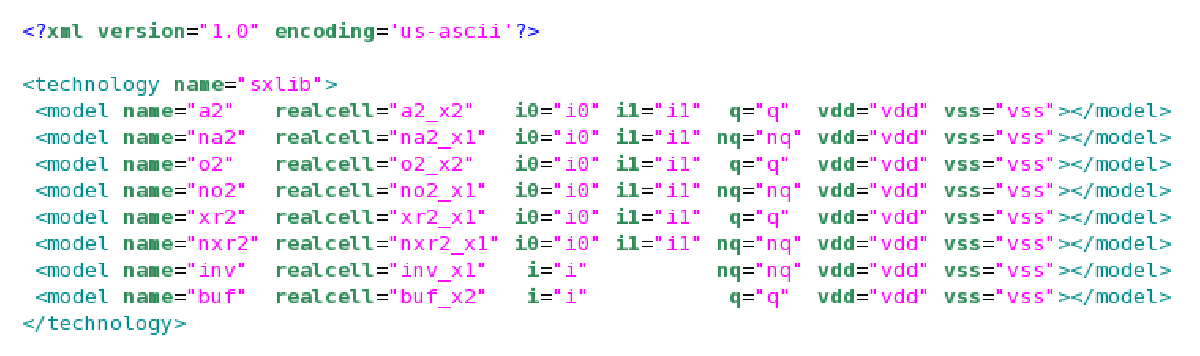
\includegraphics[width=\textwidth]{images/xml}}
          {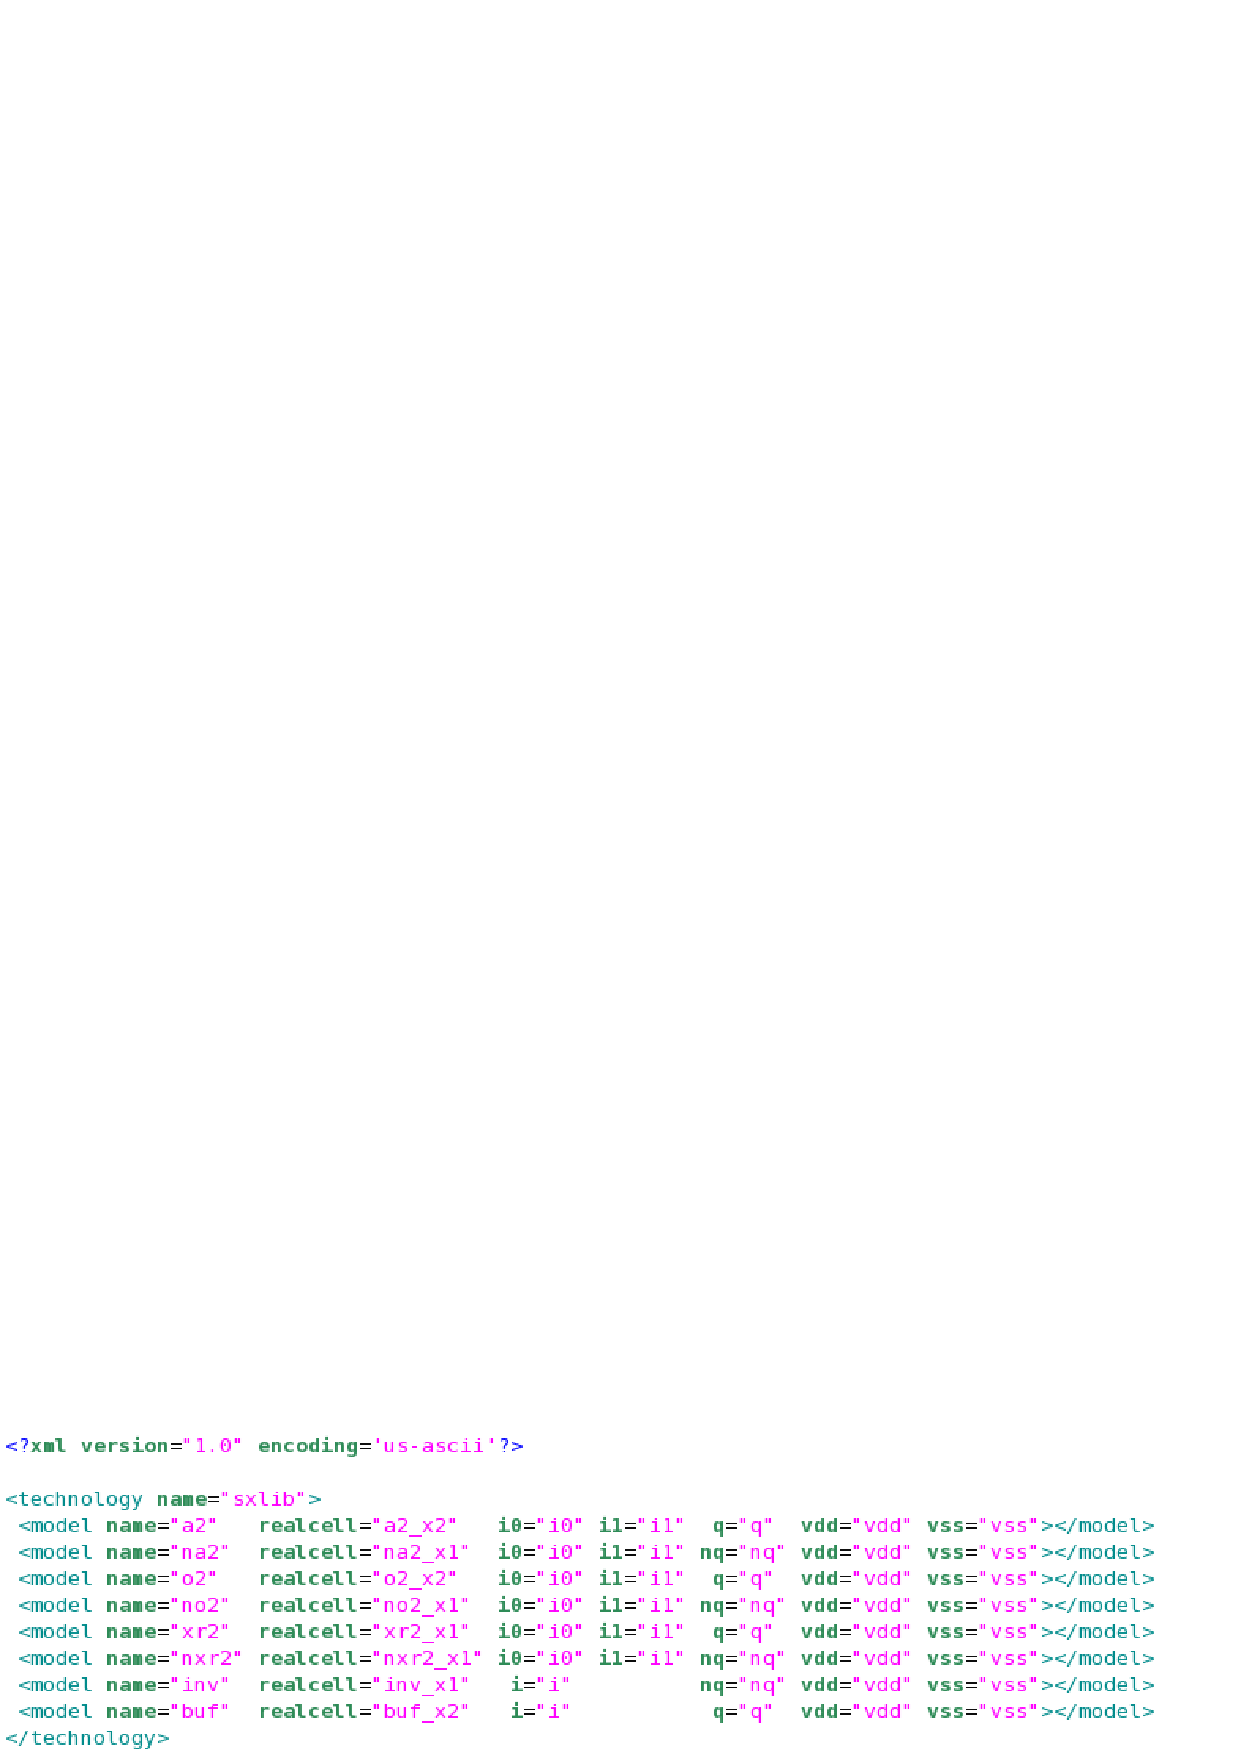
\includegraphics[width=\textwidth]{images/xml.png}}
\end{figure}

\subsubsection{Generators}

Some generators are also provided in order to use the cells of the library with nets of more than 1 bit. One has to upper the first letter of the model name in order to user those generators. What is simply done is a for loop with the bits of the nets. The parameter \verb-'nbit'- gives the size of the generator.

\subsubsection{Example}

\begin{itemize}
    \item Direct instanciation of a cell
\end{itemize}
\begin{verbatim}
for i in range ( 4 ) :
  Inst ( 'a2'
       , map = { 'i0'  : neti0[i]
               , 'i1'  : neti1[i]
               , 'q'   : netq[i]
               , 'vdd' : netvdd
               , 'vss' : netvss
               }
       )
\end{verbatim}

\begin{itemize}
    \item Instanciation of a generator
\end{itemize}
\begin{verbatim}
Generate ( 'A2', "my_and2_4bits", param = { 'nbit' : 4 } )
Inst ( 'my_and2_4bits'
     , map  = { 'i0'  : neti0
              , 'i1'  : neti1
              , 'q'   : netq
              , 'vdd' : vdd
              , 'vss' : vss
              }
     )
\end{verbatim}

\subsubsection{Errors}
    
Some errors may occur :
\begin{itemize}
    \item \verb-[Stratus ERROR] Inst : the model ... does not exist.-\\\verb-Check CRL_CATA_LIB.-\\The model of the cell has not been found. One has to check the environment variable.
    \item \verb-[Stratus ERROR] Virtual library : No file found in order to parse.-\\\verb-Check STRATUS_MAPPING_NAME.-\\The mapping file is not given in the environment variable.
\end{itemize} 

\begin{htmlonly}
\subsubsection{See Also}

\hyperref[ref]{\emph{Introduction}}{}{Introduction}{secintroduction}

\end{htmlonly}

    
    \subsection{DPGEN generators}
   
        \subsubsection{DpgenInv} 
        \begin{itemize}
    \item Name : DpgenInv -- Inverter Macro-Generator
    \item Description : Generates a \verb-n- bits inverter with an output power of \verb-drive- named \verb-modelname-.
    \begin{itemize}
        \item Valid drive are : 1, 2, 4 or 8
    \end{itemize}
    \item Terminal Names :
    \begin{itemize}
        \item \verb-i0- : input (\verb-n- bits)
        \item \verb-nq- : output (\verb-n- bits)
        \item \verb-vdd- : power
        \item \verb-vss- : ground
    \end{itemize}
    \item Parameters : Parameters are given with a map called \verb-param-.
    \begin{itemize}
        \item nbit : Defines the size of the generator
        \item drive (optional) : Defines the output power of the gates\\If this parameter is not defined, the \verb-drive- is the smallest one permitted.
    \end{itemize}
    \item Behavior :
\begin{verbatim}
nq <= not ( i0 )
\end{verbatim}
    \item Example :
\begin{verbatim}
class myClass ( Model ) :
  def Interface ( self ) :
    self._in    = LogicIn  (  "in", 32 )
    
    self._out   = LogicOut ( "out", 32 )

    self._vdd   = VddIn    ( "vdd" )
    self._vss   = VssIn    ( "vss" )
    
  def Netlist ( self ) :
      
    Inst ( 'DpgenInv'
         , param = { 'nbit' : 32 }
         , map  = { 'i0'  : self._in
                  , 'nq'  : self._out
                  , 'vdd' : self._vdd
                  , 'vss' : self._vss
                  }
         )
\end{verbatim}
\end{itemize}

        \subsubsection{DpgenBuff} 
        \begin{itemize}
    \item \textbf{Name} : DpgenBuff -- Buffer Macro-Generator
    \item \textbf{Synopsys} :
\begin{verbatim}
Generate ( 'DpgenBuff', modelname
         , param = { 'nbit'       : n
                   , 'drive'      : d
                   , 'physical'   : True
                   , 'behavioral' : True                   
                   }
         )
\end{verbatim}
    \item \textbf{Description} : Generates a \verb-n- bits inverter with an output power of \verb-d- named \verb-modelname-.
    \item \textbf{Terminal Names} :
    \begin{itemize}
        \item \textbf{i0} : input (\verb-n- bits)
        \item \textbf{q} : output (\verb-n- bits)
        \item \textbf{vdd} : power
        \item \textbf{vss} : ground
    \end{itemize}
    \item \textbf{Parameters} : Parameters are given in the map \verb-param-.
    \begin{itemize}
        \item \textbf{nbit} (mandatory) : Defines the size of the generator
        \item \textbf{drive} (optional) : Defines the output power of the gates
        \begin{itemize}
            \item Valid drive are : 2, 4 or 8
            \item If this parameter is not defined, it's value is the smallest one permitted
        \end{itemize}
        \item \textbf{physical} (optional, default value : False) : In order to generate a layout
        \item \textbf{behavioral} (optional, default value : False) : In order to generate a behavior        
    \end{itemize}
    \item \textbf{Behavior} :
\begin{verbatim}
nq <= i0
\end{verbatim}
    \item \textbf{Example} :
\begin{verbatim}
from stratus import *

class inst_buff ( Model ) :

  def Interface ( self ) :
    self.i = SignalIn  ( "i", 32 )
    self.o = SignalOut ( "o", 32 )

    self.vdd = VddIn ( "vdd" )
    self.vss = VssIn ( "vss" )
    
  def Netlist ( self ) :
    Generate ( 'DpgenBuff', 'buff_32'
             , param = { 'nbit'     : 32
                       , 'physical' : True
                       }
             )
    self.I = Inst ( 'buff_32', 'inst'
                  , map = { 'i0'  : self.i
                          , 'q'   : self.o
                          , 'vdd' : self.vdd
                          , 'vss' : self.vss
                          }
                  )
      
  def Layout ( self ) :
    Place ( self.I, NOSYM, Ref(0, 0) )
\end{verbatim}
\end{itemize}

        \subsubsection{DpgenNand2} 
        \input{man_dpgennand2}
        \subsubsection{DpgenNand3} 
        \begin{itemize}
    \item \textbf{Name} : DpgenNand3 -- Nand3 Macro-Generator
    \item \textbf{Synopsys} :
\begin{verbatim}
Generate ( 'DpgenNand3', modelname
         , param = { 'nbit'       : n
                   , 'drive'      : d
                   , 'physical'   : True
                   , 'behavioral' : True                   
                   }
         )
\end{verbatim}
    \item \textbf{Description} : Generates a \verb-n- bits three inputs NAND with an output power of \verb-d- named \verb-modelname-.
    \item \textbf{Terminal Names} :
    \begin{itemize}
        \item \textbf{i0} : input (\verb-n- bits)
        \item \textbf{i1} : input (\verb-n- bits)
        \item \textbf{i2} : input (\verb-n- bits)
        \item \textbf{nq} : output (\verb-n- bits)
        \item \textbf{vdd} : power
        \item \textbf{vss} : ground
    \end{itemize}
    \item \textbf{Parameters} : Parameters are given in the map \verb-param-.
    \begin{itemize}
        \item \textbf{nbit} (mandatory) : Defines the size of the generator
        \item \textbf{drive} (optional) : Defines the output power of the gates
        \begin{itemize}
            \item Valid drive are : 1 or 4
            \item If this parameter is not defined, it's value is the smallest one permitted
        \end{itemize}
        \item \textbf{physical} (optional, default value : False) : In order to generate a layout
        \item \textbf{behavioral} (optional, default value : False) : In order to generate a behavior
    \end{itemize}
    \item \textbf{Behavior} :
\begin{verbatim}
nq <= not ( i0 and i1 and i2 )
\end{verbatim}
    \item \textbf{Example} :
\begin{verbatim}
from stratus import *

class inst_nand3 ( Model ) :

  def Interface ( self ) :
    self.in1 = SignalIn  ( "in1", 20 )
    self.in2 = SignalIn  ( "in2", 20 )
    self.in3 = SignalIn  ( "in3", 20 )
    self.o   = SignalOut (   "o", 20 )

    self.vdd = VddIn ( "vdd" )
    self.vss = VssIn ( "vss" )
    
  def Netlist ( self ) :
    Generate ( 'DpgenNand3', 'nand3_20'
             , param = { 'nbit'     : 20
                       , 'physical' : True
                       }
             )
    self.I = Inst ( 'nand3_20', 'inst'
                  , map = { 'i0'  : self.in1
                          , 'i1'  : self.in2
                          , 'i2'  : self.in3
                          , 'nq'  : self.o
                          , 'vdd' : self.vdd
                          , 'vss' : self.vss
                          }
                  )
    
  def Layout ( self ) :
    Place ( self.I, NOSYM, Ref(0, 0) )
\end{verbatim}
\end{itemize}

        \subsubsection{Dpgennand4}
        \begin{itemize}
    \item \textbf{Name} : DpgenNand4 -- Nand4 Macro-Generator
    \item \textbf{Synopsys} :
\begin{verbatim}
Generate ( 'DpgenNand4', modelname
         , param = { 'nbit'       : n
                   , 'drive'      : d
                   , 'physical'   : True
                   , 'behavioral' : True                   
                   }
         )
\end{verbatim}
    \item \textbf{Description} : Generates a \verb-n- bits four inputs NAND with an output power of \verb-d- named \verb-modelname-.
    \item \textbf{Terminal Names} :
    \begin{itemize}
        \item \textbf{i0} : input (\verb-n- bits)
        \item \textbf{i1} : input (\verb-n- bits)
        \item \textbf{i2} : input (\verb-n- bits)
        \item \textbf{i3} : input (\verb-n- bits)
        \item \textbf{nq} : output (\verb-n- bits)
        \item \textbf{vdd} : power
        \item \textbf{vss} : ground
    \end{itemize}
    \item \textbf{Parameters} : Parameters are given in the map \verb-param-.
    \begin{itemize}
        \item \textbf{nbit} (mandatory) : Defines the size of the generator
        \item \textbf{drive} (optional) : Defines the output power of the gates
        \begin{itemize}
            \item Valid drive are : 1 or 4
            \item If this parameter is not defined, it's value is the smallest one permitted
        \end{itemize}
        \item \textbf{physical} (optional, default value : False) : In order to generate a layout
        \item \textbf{behavioral} (optional, default value : False) : In order to generate a behavior        
    \end{itemize}
    \item \textbf{Behavior} :
\begin{verbatim}
nq <= not ( i0 and i1 and i2 and i3 )
\end{verbatim}
    \item \textbf{Example} :
\begin{verbatim}
from stratus import *

class inst_nand4 ( Model ) :

  def Interface ( self ) :
    self.in1 = SignalIn  ( "in1", 9 )
    self.in2 = SignalIn  ( "in2", 9 )
    self.in3 = SignalIn  ( "in3", 9 )
    self.in4 = SignalIn  ( "in4", 9 )
    self.o   = SignalOut (   "o", 9 )

    self.vdd = VddIn ( "vdd" )
    self.vss = VssIn ( "vss" )
    
  def Netlist ( self ) :
    Generate ( 'DpgenNand4', 'nand4_9'
             , param = { 'nbit'     : 9
                       , 'physical' : True
                       }
             )
    self.I = Inst ( 'nand4_9', 'inst'
                  , map = { 'i0'  : self.in1
                          , 'i1'  : self.in2
                          , 'i2'  : self.in3
                          , 'i3'  : self.in4
                          , 'nq'  : self.o
                          , 'vdd' : self.vdd
                          , 'vss' : self.vss
                          }
                  )
    
  def Layout ( self ) :
    Place ( self.I, NOSYM, Ref(0, 0) )
\end{verbatim}
\end{itemize}

        \subsubsection{DpgenAnd2}
        \input{man_dpgenand2}
        \subsubsection{DpgenAnd3} 
        \begin{itemize}
    \item \textbf{Name} : DpgenAnd3 -- And3 Macro-Generator
    \item \textbf{Synopsys} :
\begin{verbatim}
Generate ( 'DpgenAnd3', modelname
         , param = { 'nbit'       : n
                   , 'drive'      : d
                   , 'physical'   : True
                   , 'behavioral' : True
                   }
         )
\end{verbatim}
    \item \textbf{Description} : Generates a \verb-n- bits three inputs AND with an output power of \verb-d- named \verb-modelname-.
    \item \textbf{Terminal Names} :
    \begin{itemize}
        \item \textbf{i0} : input (\verb-n- bits)
        \item \textbf{i1} : input (\verb-n- bits)
        \item \textbf{i2} : input (\verb-n- bits)
        \item \textbf{q} : output (\verb-n- bits)
        \item \textbf{vdd} : power
        \item \textbf{vss} : ground
    \end{itemize}
    \item \textbf{Parameters} : Parameters are given in the map \verb-param-.
    \begin{itemize}
        \item \textbf{nbit} (mandatory) : Defines the size of the generator
        \item \textbf{drive} (optional): Defines the output power of the gates
        \begin{itemize}
            \item Valid drive are : 2 or 4
            \item If this parameter is not defined, it's value is the smallest one permitted
        \end{itemize}
        \item \textbf{physical} (optional, default value : False): In order to generate a layout
        \item \textbf{behavioral} (optional, default value : False): In order to generate a behavior
    \end{itemize}
    \item \textbf{Behavior} :
\begin{verbatim}
nq <= i0 and i1 and i2
\end{verbatim}
    \item \textbf{Example} :
\begin{verbatim}
from stratus import *

class inst_and3 ( Model ) :

  def Interface ( self ) :
    self.in1 = SignalIn  ( "in1", 16 )
    self.in2 = SignalIn  ( "in2", 16 )
    self.in3 = SignalIn  ( "in3", 16 )
    self.out = SignalOut (   "o", 16 )

    self.vdd = VddIn ( "vdd" )
    self.vss = VssIn ( "vss" )
    
  def Netlist ( self ) :
    Generate ( 'DpgenAnd3', "and3_16"
             , param = { 'nbit'     : 16
                       , 'physical' : True
                       }
             )       
    self.I = Inst ( 'and3_16', 'inst'
                  , map = { 'i0'  : self.in1
                          , 'i1'  : self.in2
                          , 'i2'  : self.in3
                          , 'q'   : self.out
                          , 'vdd' : self.vdd
                          , 'vss' : self.vss
                          }
                  )
    
  def Layout ( self ) :
    Place ( self.I, NOSYM, Ref (0, 0) )
\end{verbatim}
\end{itemize}

        \subsubsection{DpgenAnd4} 
        \begin{itemize}
    \item Name : DpgenAnd4 -- And4 Macro-Generator
    \item Description : Generates a \verb-n- bits four inputs AND with an output power of \verb-drive- named \verb-modelname-.
    \begin{itemize}
        \item Valid drive are : 2 or 4
    \end{itemize}
    \item Terminal Names :
    \begin{itemize}
        \item i0 : input (\verb-n- bits)
        \item i1 : input (\verb-n- bits)
        \item i2 : input (\verb-n- bits)
        \item i3 : input (\verb-n- bits)
        \item q : output (\verb-n- bits)
        \item vdd : power
        \item vss : ground
    \end{itemize}
    \item Parameters : Parameters are given with a map called \verb-param-.
    \begin{itemize}
        \item nbit : Defines the size of the generator
        \item drive (optional) : Defines the output power of the gates\\If this parameter is not defined, the \verb-drive- is the smallest one permitted.
    \end{itemize}
    \item Behavior :
\begin{verbatim}
nq <= i0 and i1 and i2 and i3
\end{verbatim}
    \item Example :
\begin{verbatim}
class myClass ( Model ) :
  def Interface ( self ) :
    self._in0   = LogicIn  ( "in0", 32 )
    self._in1   = LogicIn  ( "in1", 32 )
    self._in2   = LogicIn  ( "in2", 32 )
    self._in3   = LogicIn  ( "in3", 32 )
    
    self._out   = LogicOut ( "out", 32 )

    self._vdd   = VddIn    ( "vdd" )
    self._vss   = VssIn    ( "vss" )
    
  def Netlist ( self ) :
      
    Inst ( 'DpgenAnd4'
         , param = { 'nbit' : 32 }
         , map  = { 'i0'  : self._in0
                  , 'i1'  : self._in1
                  , 'i2'  : self._in2
                  , 'i3'  : self._in3
                  , 'q'   : self._out
                  , 'vdd' : self._vdd
                  , 'vss' : self._vss
                  }
         )
\end{verbatim}
\end{itemize}

        \subsubsection{DpgenNor2} 
        \begin{itemize}
    \item \textbf{Name} : DpgenNor2 -- Nor2 Macro-Generator
    \item \textbf{Synopsys} :
\begin{verbatim}
Generate ( 'DpgenNor2', modelname
         , param = { 'nbit'       : n
                   , 'drive'      : d
                   , 'physical'   : True
                   , 'behavioral' : True                   
                   }
         )
\end{verbatim}
    \item \textbf{Description} : Generates a \verb-n- bits two inputs NOR with an output power of \verb-d- named \verb-modelname-.
    \item \textbf{Terminal Names} :
    \begin{itemize}
        \item \textbf{i0} : input (\verb-n- bits)
        \item \textbf{i1} : input (\verb-n- bits)
        \item \textbf{nq} : output (\verb-n- bits)
        \item \textbf{vdd} : power
        \item \textbf{vss} : ground
    \end{itemize}
    \item \textbf{Parameters} : Parameters are given in the map \verb-param-.
    \begin{itemize}
        \item \textbf{nbit} (mandatory) : Defines the size of the generator
        \item \textbf{drive} (optional) : Defines the output power of the gates
        \begin{itemize}
            \item Valid drive are : 1 or 4
            \item If this parameter is not defined, it's value is the smallest one permitted
        \end{itemize}
        \item \textbf{physical} (optional, default value : False) : In order to generate a layout
        \item \textbf{behavioral} (optional, default value : False) : In order to generate a behavior        
    \end{itemize}
    \item \textbf{Behavior} :
\begin{verbatim}
nq <= not ( i0 or i1 )
\end{verbatim}
    \item \textbf{Example} :
\begin{verbatim}
from stratus import *

class inst_nor2 ( Model ) :

  def Interface ( self ) :
    self.in1 = SignalIn  ( "in1", 8 )
    self.in2 = SignalIn  ( "in2", 8 )
    self.o   = SignalOut (   "o", 8 )

    self.vdd = VddIn ( "vdd" )
    self.vss = VssIn ( "vss" )
    
  def Netlist ( self ) :
    Generate ( 'DpgenNor2', 'nor2_8'
             , param = { 'nbit'     : 8
                       , 'physical' : True
                       }
             )
    self.I = Inst ( 'nor2_8', 'inst'
                  , map = { 'i0'  : self.in1
                          , 'i1'  : self.in2
                          , 'nq'  : self.o
                          , 'vdd' : self.vdd
                          , 'vss' : self.vss
                          }
                  )
    
  def Layout ( self ) :
    Place ( self.I, NOSYM, Ref(0, 0) )
\end{verbatim}
\end{itemize}

        \subsubsection{DpgenNor3} 
        \input{man_dpgennor3}
        \subsubsection{DpgenNor4} 
        \begin{itemize}
    \item \textbf{Name} : DpgenNor4 -- Nor4 Macro-Generator
    \item \textbf{Synopsys} :
\begin{verbatim}
Generate ( 'DpgenNor4', modelname
         , param = { 'nbit'       : n
                   , 'drive'      : d 
                   , 'physical'   : True
                   , 'behavioral' : True                   
                   }
         )
\end{verbatim}
    \item \textbf{Description} : Generates a \verb-n- bits four inputs NOR with an output power of \verb-d- named \verb-modelname-.
    \item \textbf{Terminal Names} :
    \begin{itemize}
        \item \textbf{i0} : input (\verb-n- bits)
        \item \textbf{i1} : input (\verb-n- bits)
        \item \textbf{i2} : input (\verb-n- bits)
        \item \textbf{i3} : input (\verb-n- bits)
        \item \textbf{nq} : output (\verb-n- bits)
        \item \textbf{vdd} : power
        \item \textbf{vss} : ground
    \end{itemize}
    \item \textbf{Parameters} : Parameters are given in the map \verb-param-.
    \begin{itemize}
        \item \textbf{nbit} (mandatory) : Defines the size of the generator
        \item \textbf{drive} (optional) : Defines the output power of the gates
        \begin{itemize}
            \item Valid drive are : 1 or 4
            \item If this parameter is not defined, it's value is the smallest one permitted
        \end{itemize}
        \item \textbf{physical} (optional, default value : False) : In order to generate a layout
        \item \textbf{behavioral} (optional, default value : False) : In order to generate a behavior        
    \end{itemize}
    \item \textbf{Behavior} :
\begin{verbatim}
nq <= not ( i0 or i1 or i2 or i3 )
\end{verbatim}
    \item \textbf{Example} :
\begin{verbatim}
from stratus import *

class inst_nor4 ( Model ) :

  def Interface ( self ) :
    self.in1 = SignalIn  ( "in1", 15 )
    self.in2 = SignalIn  ( "in2", 15 )
    self.in3 = SignalIn  ( "in3", 15 )
    self.in4 = SignalIn  ( "in4", 15 )
    self.out = SignalOut (   "o", 15 )

    self.vdd = VddIn ( "vdd" )
    self.vss = VssIn ( "vss" )
    
  def Netlist ( self ) :
    Generate ( 'DpgenNor4', 'nor4_15'
             , param = { 'nbit'     : 15
                       , 'physical' : True
                       }
             )
    self.I = Inst ( 'nor4_15', 'inst'
                  , map = { 'i0'  : self.in1
                          , 'i1'  : self.in2
                          , 'i2'  : self.in3
                          , 'i3'  : self.in4
                          , 'nq'  : self.out
                          , 'vdd' : self.vdd
                          , 'vss' : self.vss
                          }
                  )
      
    
  def Layout ( self ) :
    Place ( self.I, NOSYM, Ref(0, 0) )
\end{verbatim}
\end{itemize}

        \subsubsection{DpgenOr2} 
        \begin{itemize}
    \item Name : DpgenOr2 -- Or2 Macro-Generator
    \item Description : Generates a \verb-n- bits two inputs OR with an output power of \verb-drive- named \verb-modelname-.
    \begin{itemize}
        \item Valid drive are : 2 or 4
    \end{itemize}
    \item Terminal Names :
    \begin{itemize}
        \item i0 : input (\verb-n- bits)
        \item i1 : input (\verb-n- bits)
        \item q : output (\verb-n- bits)
        \item vdd : power
        \item vss : ground
    \end{itemize}
    \item Parameters : Parameters are given with a map called \verb-param-.
    \begin{itemize}
        \item nbit : Defines the size of the generator
        \item drive (optional) : Defines the output power of the gates\\If this parameter is not defined, the \verb-drive- is the smallest one permitted.
    \end{itemize}
    \item Behavior :
\begin{verbatim}
nq <= i0 or i1
\end{verbatim}
    \item Example :
\begin{verbatim}
class myClass ( Model ) :
  def Interface ( self ) :
    self._in0   = LogicIn  ( "in0", 32 )
    self._in1   = LogicIn  ( "in1", 32 )
    
    self._out   = LogicOut ( "out", 32 )

    self._vdd   = VddIn    ( "vdd" )
    self._vss   = VssIn    ( "vss" )
    
  def Netlist ( self ) :
      
    Inst ( 'DpgenOr2'
         , param = { 'nbit' : 32 }
         , map  = { 'i0'  : self._in0
                  , 'i1'  : self._in1
                  , 'q'   : self._out
                  , 'vdd' : self._vdd
                  , 'vss' : self._vss
                  }
         )
\end{verbatim}
\end{itemize}

        \subsubsection{DpgenOr3} 
        \begin{itemize}
    \item \textbf{Name} : DpgenOr3 -- Or3 Macro-Generator
    \item \textbf{Synopsys} :
\begin{verbatim}
Generate ( 'DpgenOr3', modelname
         , param = { 'nbit'       : n
                   , 'drive'      : d
                   , 'physical'   : True
                   , 'behavioral' : True                   
                   }
         )
\end{verbatim}
    \item \textbf{Description} : Generates a \verb-n- bits three inputs OR with an output power of \verb-d- named \verb-modelname-.
    \item \textbf{Terminal Names} :
    \begin{itemize}
        \item \textbf{i0} : input (\verb-n- bits)
        \item \textbf{i1} : input (\verb-n- bits)
        \item \textbf{i2} : input (\verb-n- bits)
        \item \textbf{q} : output (\verb-n- bits)
        \item \textbf{vdd} : power
        \item \textbf{vss} : ground
    \end{itemize}
    \item \textbf{Parameters} : Parameters are given in the map \verb-param-.
    \begin{itemize}
        \item \textbf{nbit} (mandatory) : Defines the size of the generator
        \item \textbf{drive} (optional) : Defines the output power of the gates
        \begin{itemize}
            \item Valid drive are : 2 or 4
            \item If this parameter is not defined, it's value is the smallest one permitted
        \end{itemize}
        \item \textbf{physical} (optional, default value : False) : In order to generate a layout
        \item \textbf{behavioral} (optional, default value : False) : In order to generate a behavior        
    \end{itemize}
    \item \textbf{Behavior} :
\begin{verbatim}
nq <= i0 or i1 or i2
\end{verbatim}
    \item \textbf{Example} :
\begin{verbatim}
from stratus import *

class inst_or3 ( Model ) :

  def Interface ( self ) :
    self.in1 = SignalIn  ( "in1", 5 )
    self.in2 = SignalIn  ( "in2", 5 )
    self.in3 = SignalIn  ( "in3", 5 )
    self.o   = SignalOut (   "o", 5 )

    self.vdd = VddIn ( "vdd" )
    self.vss = VssIn ( "vss" )
    
  def Netlist ( self ) :
    Generate ( 'DpgenOr3', 'or3_5'
             , param = { 'nbit'     : 5 
                       , 'physical' : True
                       }
             )
    self.I = Inst ( 'or3_5', 'inst'
                  , map = { 'i0'  : self.in1
                          , 'i1'  : self.in2
                          , 'i2'  : self.in3
                          , 'q'   : self.o
                          , 'vdd' : self.vdd
                          , 'vss' : self.vss
                          }
                  )
    
  def Layout ( self ) :
    Place ( self.I, NOSYM, Ref(0, 0) )
\end{verbatim}
\end{itemize}

        \subsubsection{DpgenOr4} 
        \input{man_dpgenor4}
        \subsubsection{DpgenXor2} 
        \begin{itemize}
    \item \textbf{Name} : DpgenXor2 -- Xor2 Macro-Generator
    \item \textbf{Synopsys} :
\begin{verbatim}
Generate ( 'DpgenXor2', modelname
         , param = { 'nbit'       : n
                   , 'drive'      : d
                   , 'physical'   : True
                   , 'behavioral' : True                   
                   }
         )
\end{verbatim}
    \item \textbf{Description} : Generates a \verb-n- bits two inputs XOR with an output power of \verb-d- named \verb-modelname-.
    \item \textbf{Terminal Names} :
    \begin{itemize}
        \item \textbf{i0} : input (\verb-n- bits)
        \item \textbf{i1} : input (\verb-n- bits)
        \item \textbf{q} : output (\verb-n- bits)
        \item \textbf{vdd} : power
        \item \textbf{vss} : ground
    \end{itemize}
    \item \textbf{Parameters} : Parameters are given in the map \verb-param-.
    \begin{itemize}
        \item \textbf{nbit} (mandatory) : Defines the size of the generator
        \item \textbf{drive} (optional) : Defines the output power of the gates
        \begin{itemize}
            \item Valid drive are : 2 or 4
            \item If this parameter is not defined, it's value is the smallest one permitted
        \end{itemize}
        \item \textbf{physical} (optionnal, default value : False) : In order to generate a layout
        \item \textbf{behavioral} (optionnal, default value : False) : In order to generate a behavior        
    \end{itemize}
    \item \textbf{Behavior} :
\begin{verbatim}
nq <= i0 xor i1
\end{verbatim}
    \item \textbf{Example} :
\begin{verbatim}
from stratus import *

class inst_xor2 ( Model ) :

  def Interface ( self ) :
    self.in1 = SignalIn  ( "in1", 8 )
    self.in2 = SignalIn  ( "in2", 8 )
    self.o   = SignalOut (   "o", 8 )

    self.vdd = VddIn ( "vdd" )
    self.vss = VssIn ( "vss" )
    
  def Netlist ( self ) :
    Generate ( 'DpgenXor2', 'xor2_8'
             , param = { 'nbit' : 8 
                       , 'physical' : True
                       }
             )
    self.I = Inst ( 'xor2_8', 'inst'
                  , map = { 'i0'  : self.in1
                          , 'i1'  : self.in2
                          , 'q'   : self.o
                          , 'vdd' : self.vdd
                          , 'vss' : self.vss
                          }
                  )
    
  def Layout ( self ) :
    Place ( self.I, NOSYM, Ref(0, 0) )
\end{verbatim}
\end{itemize}

        \subsubsection{DpgenXnor2} 
        \input{man_dpgenxnor2}
        \subsubsection{DpgenNmux2}
        \begin{itemize}
    \item \textbf{Name} : DpgenNmux2 -- Multiplexer Macro-Generator
    \item \textbf{Synopsys} :
\begin{verbatim}
Generate ( 'DpgenNmux2', modelname
         , param = { 'nbit'       : n
                   , 'physical'   : True
                   , 'behavioral' : True         
                   }
         )
\end{verbatim}
    \item \textbf{Description} : Generates a \verb-n- bits two inputs multiplexer named \verb-modelname-.
    \item \textbf{Terminal Names} :
    \begin{itemize}
        \item \textbf{cmd} : select ( 1 bit )
        \item \textbf{i0} : input ( \verb-n- bits )
        \item \textbf{i1} : input ( \verb-n- bits )
        \item \textbf{nq} : output ( \verb-n- bits )
        \item \textbf{vdd} : power
        \item \textbf{vss} : ground
    \end{itemize}
    \item \textbf{Parameters} : Parameters are given in the map \verb-param-.
    \begin{itemize}
        \item \textbf{nbit} (mandatory) : Defines the size of the generator
        \item \textbf{physical} (optional, default value : False) : In order to generate a layout
        \item \textbf{behavioral} (optional, default value : False) : In order to generate a behavior
    \end{itemize}
    \item \textbf{Behavior} :
\begin{verbatim}
nq <= WITH cmd SELECT not i0 WHEN '0',
                      not i1 WHEN '1';
\end{verbatim}
    \item \textbf{Example} :
\begin{verbatim}
from stratus import *

class inst_nmux2 ( Model ) :

  def Interface ( self ) :
    self.in1 = SignalIn  (  "in1", 5 )
    self.in2 = SignalIn  (  "in2", 5 )
    self.cmd = SignalIn  (  "cmd", 1 )
    self.o   = SignalOut (    "o", 5 )

    self.vdd = VddIn ( "vdd" )
    self.vss = VssIn ( "vss" )
    
  def Netlist ( self ) :
    Generate ( 'DpgenNmux2', 'nmux2_5'
             , param = { 'nbit'     : 5
                       , 'physical' : True
                       }
             )
    self.I = Inst ( 'nmux2_5', 'inst'
                  , map = { 'i0'  : self.in1
                          , 'i1'  : self.in2
                          , 'cmd' : self.cmd
                          , 'nq'  : self.o
                          , 'vdd' : self.vdd
                          , 'vss' : self.vss
                          }
                  )
      
  def Layout ( self ) :
    Place ( self.I, NOSYM, Ref(0, 0) )
\end{verbatim}
\end{itemize}

        \subsubsection{DpgenMux2}
        \begin{itemize}
    \item \textbf{Name} : DpgenMux2 -- Multiplexer Macro-Generator
    \item \textbf{Synopsys} :
\begin{verbatim}
Generate ( 'DpgenMux2', modelname
         , param = { 'nbit'       : n
                   , 'drive'      : d
                   , 'physical'   : True
                   , 'behavioral' : True                   
                   }
         )
\end{verbatim}
    \item \textbf{Description} : Generates a \verb-n- bits two inputs multiplexer with an output power of \verb-d- named \verb-modelname-.
    \item \textbf{Terminal Names} :
    \begin{itemize}
        \item \textbf{cmd} : select ( 1 bit )
        \item \textbf{i0} : input ( \verb-n- bits )
        \item \textbf{i1} : input ( \verb-n- bits )
        \item \textbf{q} : output ( \verb-n- bits )
        \item \textbf{vdd} : power
        \item \textbf{vss} : ground
    \end{itemize}
    \item \textbf{Parameters} : Parameters are given in the map \verb-param-.
    \begin{itemize}
        \item \textbf{nbit} (mandatory) : Defines the size of the generator
        \item \textbf{nbit\_cmd} (mandatory) : Defines the size of the generator
        \item \textbf{drive} (optional) : Defines the output power of the gates
        \begin{itemize}
            \item Valid drive are : 2 or 4
            \item If this parameter is not defined, it's value is the smallest one permitted
        \end{itemize}
        \item \textbf{physical} (optional, default value : False) : In order to generate a layout
        \item \textbf{behavioral} (optional, default value : False) : In order to generate a behavior        
    \end{itemize}
    \item \textbf{Behavior} :
\begin{verbatim}
nq <= WITH cmd SELECT i0 WHEN '0',
                      i1 WHEN '1';
\end{verbatim}
    \item \textbf{Example} :
\begin{verbatim}
from stratus import *

class inst_mux2 ( Model ) :

  def Interface ( self ) :
    self.in1  = SignalIn  ( "in1", 8 )
    self.in2  = SignalIn  ( "in2", 8 )
    self.cmd  = SignalIn  ( "cmd", 1 )
    self.o    = SignalOut (   "o", 8 )

    self.vdd = VddIn ( "vdd" )
    self.vss = VssIn ( "vss" )
    
  def Netlist ( self ) :
    Generate ( 'DpgenMux2', 'mux2_8'
             , param = { 'nbit'     : 8
                       , 'physical' : True
                       }
             )
    self.I = Inst ( 'mux2_8', 'inst'
                  , map = { 'i0'  : self.in1
                          , 'i1'  : self.in2
                          , 'cmd' : self.cmd
                          , 'q'   : self.o
                          , 'vdd' : self.vdd
                          , 'vss' : self.vss
                          }
                  )
    
  def Layout ( self ) :
    Place ( self.I, NOSYM, Ref(0, 0) )
\end{verbatim}
\end{itemize}

        \subsubsection{DpgenNbuse} 
        \begin{itemize}
    \item Name : DpgenNbuse -- Tristate Macro-Generator
    \item Description : Generates a \verb-n- bits tristate with an complemented output named \verb-modelname-.
    \item Terminal Names :
    \begin{itemize}
        \item cmd : select ( 1 bit )
        \item i0 : input ( \verb-n- bits )
        \item nq : output ( \verb-n- bits )
        \item vdd : power
        \item vss : ground
    \end{itemize}
    \item Parameters : Parameters are given with a map called \verb-param-.
    \begin{itemize}
        \item nbit : Defines the size of the generator
    \end{itemize}
    \item Behavior :
\begin{verbatim}
nts:BLOCK(cmd = '1') BEGIN
    nq <= GUARDED not(i0);
END
\end{verbatim}
    \item Example :
\begin{verbatim}
class myClass ( Model ) :
  def Interface ( self ) :
    self._in    = LogicIn  (  "in", 32 )
    self._cmd   = LogicIn  ( "cmd", 1 )
    
    self._out   = TriState ( "out", 32 )

    self._vdd   = VddIn    ( "vdd" )
    self._vss   = VssIn    ( "vss" )
    
  def Netlist ( self ) :
      
    Inst ( 'DpgenNbuse'
         , param = { 'nbit' : 32 }
         , map  = { 'i0'      : self._in
                  , 'cmd'     : self._cmd
                  , 'nq'      : self._out
                  , 'vdd'     : self._vdd
                  , 'vss'     : self._vss
                  }
         )
\end{verbatim}
\end{itemize}

        \subsubsection{DpgenBuse}
        \begin{itemize}
    \item Name : DpgenBuse -- Tristate Macro-Generator
    \item Description : Generates a \verb-n- bits tristate with an output power of \verb-drive- named \verb-modelname-.
    \begin{itemize}
        \item Valid drive are : 4 or 8
    \end{itemize}
    \item Terminal Names :
    \begin{itemize}
        \item cmd : select ( 1 bit )
        \item i0 : input ( \verb-n- bits )
        \item q : output ( \verb-n- bits )
        \item vdd : power
        \item vss : ground
    \end{itemize}
    \item Parameters : Parameters are given with a map called \verb-param-.
    \begin{itemize}
        \item nbit : Defines the size of the generator
    \end{itemize}
    \item Behavior :
\begin{verbatim}
nts:BLOCK(cmd = '1') BEGIN
    q <= GUARDED i0;
END
\end{verbatim}
    \item Example :
\begin{verbatim}
class myClass ( Model ) :
  def Interface ( self ) :
    self._in    = LogicIn  (  "in", 32 )
    self._cmd   = LogicIn  ( "cmd", 1 )
    
    self._out   = TriState ( "out", 32 )

    self._vdd   = VddIn    ( "vdd" )
    self._vss   = VssIn    ( "vss" )
    
  def Netlist ( self ) :
      
    Inst ( 'DpgenBuse'
         , param = { 'nbit' : 32 }
         , map  = { 'i0'      : self._in
                  , 'cmd'     : self._cmd
                  , 'q'       : self._out
                  , 'vdd'     : self._vdd
                  , 'vss'     : self._vss
                  }
         )
\end{verbatim}
\end{itemize}

        \subsubsection{DpgenNand2mask} 
        \begin{itemize}
    \item \textbf{Name} : DpgenNand2mask -- Programmable Mask Macro-Generator
    \item \textbf{Synopsys} :
\begin{verbatim}
Generate ( 'DpgenNand2mask', modelname
         , param = { 'nbit'       : n
                   , 'const'      : constVal
                   , 'physical'   : True
                   , 'behavioral' : True                   
                   }
         )
\end{verbatim}
    \item \textbf{Description} : Generates a \verb-n- bits conditionnal NAND mask named \verb-modelname-.
    \item \textbf{Terminal Names} :
    \begin{itemize}
        \item \textbf{cmd} : mask control ( 1 bit )
        \item \textbf{i0} : input ( \verb-n- bits )
        \item \textbf{nq} : output ( \verb-n- bits )
        \item \textbf{vdd} : power
        \item \textbf{vss} : ground
    \end{itemize}
    \item \textbf{Parameters} : Parameters are given in the map \verb-param-.
    \begin{itemize}
        \item \textbf{nbit} (mandatory) : Defines the size of the generator
        \item \textbf{const} (mandatory) : Defines the constant (string beginning with 0b, 0x or 0o functions of the basis)
        \item \textbf{physical} (optional, default value : False) : In order to generate a layout
        \item \textbf{behavioral} (optional, default value : False) : In order to generate a behavior        
    \end{itemize}
    \item \textbf{How it works} :
    \begin{itemize}
        \item If the \verb-cmd- signal is set to \verb-zero-, the mask is NOT applied, so the whole operator behaves like an inverter.
        \item If the \verb-cmd- signal is set to \verb-one-, the mask is applied, the output is the \emph{complemented} result of the input value \emph{ANDed} with the mask (suplied by \verb-constVal-).
        \item The constant \verb-constVal- is given to the macro-generator call, therefore the value cannot be changed afterward : it's hard wired in the operator.
        \item A common error is to give a real constant for the \verb-constVal- argument. Be aware that it is a character string.
    \end{itemize}    
    \item \textbf{Behavior} :
\begin{verbatim}
nq <= WITH cmd SELECT not(i0)              WHEN '0',
                      not(i0 and constVal) WHEN '1';
\end{verbatim}
    \item \textbf{Example} :
\begin{verbatim}
from stratus import *

class inst_nand2mask ( Model ) :

  def Interface ( self ) :
    self.i   = SignalIn  (   "i", 32 )
    self.cmd = SignalIn  ( "cmd",  1 )
    self.o   = SignalOut (   "o", 32 )

    self.vdd = VddIn ( "vdd" )
    self.vss = VssIn ( "vss" )
    
  def Netlist ( self ) :
    Generate ( 'DpgenNand2mask', 'nand2mask_0x0000ffff'
             , param = { 'nbit'     : 32
                       , 'const'    : "0x0000FFFF"
                       , 'physical' : True
                       }
             )      
    self.I = Inst ( 'nand2mask_0x0000ffff', 'inst'
                  , map = { 'i0'  : self.i
                          , 'cmd' : self.cmd
                          , 'nq'  : self.o
                          , 'vdd' : self.vdd
                          , 'vss' : self.vss
                          }
                  )
    
  def Layout ( self ) :
    Place ( self.I, NOSYM, Ref(0, 0) )
\end{verbatim}
\end{itemize}

        \subsubsection{DpgenNor2mask} 
        \input{man_dpgennor2mask}
        \subsubsection{DpgenXnor2mask} 
        \begin{itemize}
    \item \textbf{Name} : DpgenXnor2mask -- Programmable Mask Macro-Generator
    \item \textbf{Synopsys} :
\begin{verbatim}
Generate ( 'DpgenXnor2mask', modelname
         , param = { 'nbit'       : n
                   , 'const'      : constVal
                   , 'physical'   : True
                   , 'behavioral' : True                   
                   }
         )
\end{verbatim}
    \item \textbf{Description} : Generates a \verb-n- bits conditionnal XNOR mask named \verb-modelname-.
    \item \textbf{Terminal Names} :
    \begin{itemize}
        \item \textbf{cmd} : mask control ( 1 bit )
        \item \textbf{i0} : input ( \verb-n- bits )
        \item \textbf{nq} : output ( \verb-n- bits )
        \item \textbf{vdd} : power
        \item \textbf{vss} : ground
    \end{itemize}
    \item \textbf{Parameters} : Parameters are given in the map \verb-param-.
    \begin{itemize}
        \item \textbf{nbit} (mandatory) : Defines the size of the generator
        \item \textbf{const} (mandatory) : Defines the constant (string beginning with 0b, 0x or 0o functions of the basis)
        \item \textbf{physical} (optional, default value : False) : In order to generate a layout
        \item \textbf{behavioral} (optional, default value : False) : In order to generate a behavior        
    \end{itemize}
    \item \textbf{How it works} :
    \begin{itemize}
        \item If the \verb-cmd- signal is set to \verb-zero-, the mask is NOT applied, so the whole operator behaves like an inverter.
        \item If the \verb-cmd- signal is set to \verb-one-, the mask is applied, the output is the \emph{complemented} result of the input value \emph{XORed} with the mask (suplied by \verb-constVal-).
        \item The constant \verb-constVal- is given to the macro-generator call, therefore the value cannot be changed afterward : it's hard wired in the operator.
        \item A common error is to give a real constant for the \verb-constVal- argument. Be aware that it is a character string.
    \end{itemize}    
    \item \textbf{Behavior} :
\begin{verbatim}
nq <= WITH cmd SELECT not(i0)              WHEN '0',
                      not(i0 xor constVal) WHEN '1';
\end{verbatim}
    \item \textbf{Example} :
\begin{verbatim}
from stratus import *

class inst_xnor2mask ( Model ) :

  def Interface ( self ) :
    self.i   = SignalIn  (   "i", 8 )
    self.cmd = SignalIn  ( "cmd", 1 )
    self.o   = SignalOut (   "o", 8 )

    self.vdd = VddIn ( "vdd" )
    self.vss = VssIn ( "vss" )
    
  def Netlist ( self ) :
    Generate ( 'DpgenXnor2mask', 'xnor2mask_0b000111'
             , param = { 'nbit'     : 8
                       , 'const'    : "0b000111"
                       , 'physical' : True
                       }
             )
    self.I = Inst ( 'xnor2mask_0b000111', 'inst'
                  , map = { 'i0'  : self.i
                          , 'cmd' : self.cmd
                          , 'nq'  : self.o
                          , 'vdd' : self.vdd
                          , 'vss' : self.vss
                          }
                  )
    
  def Layout ( self ) :
    Place ( self.I, NOSYM, Ref(0, 0) )
\end{verbatim}
\end{itemize}

        \subsubsection{DpgenAdsb2f} 
        \begin{itemize}
    \item Name : DpgenAdsb2f -- Adder/Substractor Macro-Generator
    \item Description : Generates a \verb-n- bits adder/substractor named \verb-modelname-.
    \item How it works :
    \begin{itemize}
        \item if the \verb-add_sub- signal is set to \verb-zero- an addition is performed, otherwise it's a substraction.
        \item Operation can be either signed or unsigned. In unsigned mode \verb-c31- is the overflow. in signed mode you have to compute overflow by \emph{XORing} \verb-c31- and \verb-c30-
    \end{itemize}
    \item Terminal Names :
    \begin{itemize}
        \item add\_sub : select addition or substraction (input, 1 bit)
        \item c31 : carry out. In unsigned mode, this is the overflow (output, 1 bit)
        \item c30 : used to compute overflow in signed mode : \verb-overflow = c31 xor c30- (output, 1 bit)
        \item i0 : first operand (input, \verb-n- bits)
        \item i1 : second operand (input, \verb-n- bits)
        \item q : output (\verb-n- bits)
        \item vdd : power
        \item vss : ground
    \end{itemize}
    \item Parameters : Parameters are given with a map called \verb-param-.
    \begin{itemize}
        \item nbit : Defines the size of the generator
    \end{itemize}
%    \item Behavior :
%\begin{verbatim}
%\end{verbatim}
    \item Example :
\begin{verbatim}
class myClass ( Model ) :
  def Interface ( self ) :
    self._in    = LogicIn  (  "in", 8 )
    self._in2   = LogicIn  ( "in2", 8 )
    
    self._out   = LogicOut ( "out", 8 )

    self._as    = LogicIn  (  "as", 1 )
    self._c0    = LogicOut (  "c0", 1 )
    self._c1    = LogicOut (  "c1", 1 )
    
    self._vdd   = VddIn    ( "vdd" )
    self._vss   = VssIn    ( "vss" )
    
  def Netlist ( self ) :
      
    Inst ( 'DpgenAdsb2f'
         , param = { 'nbit' : 8 }
         , map  = { 'i0'      : self._in
                  , 'i1'      : self._in2
                  , 'add_sub' : self._as
                  , 'q'       : self._out
                  , 'c30'     : self._c0
                  , 'c31'     : self._c1
                  , 'vdd'     : self._vdd
                  , 'vss'     : self._vss
                  }
         )
\end{verbatim}
\end{itemize}

        \subsubsection{DpgenShift} 
        \begin{itemize}
    \item \textbf{Name} : DpgenShift -- Shifter Macro-Generator
    \item \textbf{Synopsys} :
\begin{verbatim}
Generate ( 'DpgenShift', modelname
         , param = { 'nbit'     : n
                   , 'physical' : True         
                   }
         )
\end{verbatim}
    \item \textbf{Description} : Generates a \verb-n- bits shifter named \verb-modelname-.
    \item \textbf{Terminal Names} :
    \begin{itemize}
        \item \textbf{op} : select the kind of shift (input, 2 bits)
        \item \textbf{shamt} : the shift amount (input, \verb-Y- bits)
        \item \textbf{i} : value to shift (input, \verb-n- bits)
        \item \textbf{o} : output (\verb-n- bits)
        \item \textbf{vdd} : power
        \item \textbf{vss} : ground
    \end{itemize}
    \item \textbf{Parameters} : Parameters are given in the map \verb-param-.
    \begin{itemize}
        \item \textbf{nbit} (mandatory) : Defines the size of the generator
        \item \textbf{physical} (optional, default value : False) : In order to generate a layout
    \end{itemize}
    \item \textbf{How it works} :
    \begin{itemize}
        \item If the \verb-op[0]- signal is set to \verb-one-, performs a right shift, performs a left shift otherwise.
        \item If the \verb-op[1]- signal is set to \verb-one-, performs an arithmetic shift (only meaningful in case of a right shift).
        \item shamt : specifies the shift amount. The width of this signal (\verb-Y-) is computed from the operator's width : \verb-Y = ceil(log2(n)) -- 1
    \end{itemize}    
%    \item \textbf{Behavior} :
%\begin{verbatim}
%\end{verbatim}
    \item \textbf{Example} :
\begin{verbatim}
from stratus import *

class inst_shifter ( Model ) :

  def Interface ( self ) :
    self.instop    = SignalIn  (    "instop", 2 )
    self.instshamt = SignalIn  ( "instshamt", 2 )
    self.insti     = SignalIn  (     "insti", 4 )
    self.insto     = SignalOut (     "insto", 4 )
    
    self.vdd = VddIn ( "vdd" )
    self.vss = VssIn ( "vss" )
    
  def Netlist ( self ) :
    Generate ( 'DpgenShifter', 'shifter_4'
             , param = { 'nbit'     : 4
                       , 'physical' : True
                       }
             )
    self.I = Inst ( 'shifter_4', 'inst'
                  , map = { 'op'    : self.instop
                          , 'shamt' : self.instshamt
                          , 'i'     : self.insti
                          , 'o'     : self.insto
                          , 'vdd'   : self.vdd
                          , 'vss'   : self.vss
                          }
                  )
    
  def Layout ( self ) :
    Place ( self.I, NOSYM, Ref(0, 0) )
\end{verbatim}
\end{itemize}

        \subsubsection{DpgenShrot} 
        \begin{itemize}
    \item \textbf{Name} : DpgenShrot -- Shift/Rotation Macro-Generator
    \item \textbf{Synopsys} :
\begin{verbatim}
Generate ( 'DpgenShrot', modelname
         , param = { 'nbit'     : n
                   , 'physical' : True         
                   }
         )
\end{verbatim}
    \item \textbf{Description} : Generates a \verb-n- bits shift/rotation operator named \verb-modelname-.
    \item \textbf{Terminal Names} :
    \begin{itemize}
        \item \textbf{op} : select the kind of shift/rotation (input, 3 bits)
        \item \textbf{shamt} : the shift amount (input, \verb-Y- bits)
        \item \textbf{i} : value to shift (input, \verb-n- bits)
        \item \textbf{o} : output (\verb-n- bits)
        \item \textbf{vdd} : power
        \item \textbf{vss} : ground
    \end{itemize}
    \item \textbf{Parameters} : Parameters are given in the map \verb-param-.
    \begin{itemize}
        \item \textbf{nbit} (mandatory) : Defines the size of the generator
        \item \textbf{physical} (optional, default value : False) : In order to generate a layout        
    \end{itemize}
    \item \textbf{How it works} :
    \begin{itemize}
        \item If the \verb-op[0]- signal is set to \verb-one-, performs a right shift/rotation , otherwise left shift/rotation occurs.
        \item If the \verb-op[1]- signal is set to \verb-one-, performs an arithmetic shift (only meaningful in case of a right shift).
        \item If the \verb-op[2]- signal is set to \verb-one-, performs a rotation, otherwise performs a shift..
        \item \verb-shamt- specifies the shift amount. The width of this signal (\verb-Y-) is computed from the operator's width : \verb-Y = ceil(log2(n))- - 1
    \end{itemize}    
%    \item \textbf{Behavior} :
%\begin{verbatim}
%\end{verbatim}
    \item \textbf{Example} :
\begin{verbatim}
from stratus import *

class inst_shrot ( Model ) :

  def Interface ( self ) :
    self.rotop     = SignalIn  (     "rotop", 3 )
    self.instshamt = SignalIn  ( "instshamt", 2 )
    self.insti     = SignalIn  (     "insti", 4 )
    self.insto     = SignalOut (     "insto", 4 )
    
    self.vdd = VddIn ( "vdd" )
    self.vss = VssIn ( "vss" )
    
  def Netlist ( self ) :
    Generate ( 'DpgenShrot', 'shrot_4'
             , param = { 'nbit'     : 4
                       , 'physical' : True
                       }
             )
    self.I = Inst ( 'shrot_4', 'inst'
                  , map = { 'op'    : self.rotop
                          , 'shamt' : self.instshamt
                          , 'i'     : self.insti
                          , 'o'     : self.insto
                          , 'vdd'   : self.vdd
                          , 'vss'   : self.vss
                          }
                  )
    
  def Layout ( self ) :
    Place ( self.I, NOSYM, Ref(0, 0) )
\end{verbatim}
\end{itemize}

        \subsubsection{DpgenNul}
        \begin{itemize}
    \item Name : DpgenNul -- Zero Detector Macro-Generator
    \item Description : Generates a \verb-n- bits zero detector named \verb-modelname-.
    \item Terminal Names :
    \begin{itemize}
        \item i0 : value to check (input, \verb-n- bits)
        \item q : null flag (1 bit)
        \item vdd : power
        \item vss : ground
    \end{itemize}
    \item Parameters : Parameters are given with a map called \verb-param-.
    \begin{itemize}
        \item nbit : Defines the size of the generator
    \end{itemize}
    \item Behavior :
\begin{verbatim}
q <= '1' WHEN ( i0 = X"00000000" ) ELSE '0';
\end{verbatim}
    \item Example :
\begin{verbatim}
class myClass ( Model ) :
  def Interface ( self ) :
    self._in    = LogicIn  (  "in", 32 )
    
    self._out   = LogicOut ( "out", 1 )
    
    self._vdd   = VddIn    ( "vdd" )
    self._vss   = VssIn    ( "vss" )
    
  def Netlist ( self ) :
      
    Inst ( 'DpgenNul'
         , param = { 'nbit' : 32 }
         , map  = { 'i0'      : self._in
                  , 'nul'     : self._out
                  , 'vdd'     : self._vdd
                  , 'vss'     : self._vss
                  }
         )    
\end{verbatim}
\end{itemize}

        \subsubsection{DpgenConst}
        \begin{itemize}
    \item \textbf{Name} : DpgenConst -- Constant Macro-Generator
    \item \textbf{Synopsys} :
\begin{verbatim}
Generate ( 'DpgenConst', modelname
         , param = { 'nbit'       : n
                   , 'const'      : constVal
                   , 'physical'   : True
                   , 'behavioral' : True                   
                   }
         )
\end{verbatim}
    \item \textbf{Description} : Generates a \verb-n- bits constant named \verb-modelname-.
    \item \textbf{Terminal Names} :
    \begin{itemize}
        \item \textbf{q} : the constant (output, \verb-n- bit)
        \item \textbf{vdd} : power
        \item \textbf{vss} : ground
    \end{itemize}
    \item \textbf{Parameters} : Parameters are given in the map \verb-param-.
    \begin{itemize}
        \item \textbf{nbit } (mandatory) : Defines the size of the generator
        \item \textbf{const} (mandatory) : Defines the constant (string beginning with 0b, 0x or 0o functions of the basis)
        \item \textbf{physical} (optional, default value : False) : In order to generate a layout
        \item \textbf{behavioral} (optional, default value : False) : In order to generate a behavior
    \end{itemize}
    \item \textbf{Behavior} :
\begin{verbatim}
q <= constVal
\end{verbatim}
    \item \textbf{Example} :
\begin{verbatim}
from stratus import *

class inst_const ( Model ) :

  def Interface ( self ) :
    self.o = SignalOut ( "o", 32 )

    self.vdd = VddIn ( "vdd" )
    self.vss = VssIn ( "vss" )
    
  def Netlist ( self ) :
    Generate ( 'DpgenConst', 'const_0x0000ffff'
             , param = { 'nbit'     : 32
                       , 'const'    : "0x0000FFFF"
                       , 'physical' : True
                       }
             )      
    self.I = Inst ( 'const_0x0000ffff', 'inst'
                  , map = { 'q'   : self.o
                          , 'vdd' : self.vdd
                          , 'vss' : self.vss
                          }
                  )
      
  def Layout ( self ) :
    Place ( self.I, NOSYM, Ref(0, 0) )
\end{verbatim}
\end{itemize}

        \subsubsection{DpgenRom2}
        \begin{itemize}
    \item \textbf{Name} : DpgenRom2 -- 2 words ROM Macro-Generator
    \item \textbf{Synopsys} :
\begin{verbatim}
Generate ( 'DpgenRom2', modelname
         , param = { 'nbit'     : n
                   , 'val0'     : constVal0
                   , 'val1'     : constVal1
                   , 'physical' : True                   
                   }
         )
\end{verbatim}
    \item \textbf{Description} : Generates a \verb-n- bits 2 words optimized ROM named \verb-modelname-.
    \item \textbf{Terminal Names} :
    \begin{itemize}
        \item \textbf{sel0} : address of the value (input, 1 bit)
        \item \textbf{q} : the selected word (output, \verb-n- bits)
        \item \textbf{vdd} : power
        \item \textbf{vss} : ground
    \end{itemize}
    \item \textbf{Parameters} : Parameters are given in the map \verb-param-.
    \begin{itemize}
        \item \textbf{nbit} (mandatory) : Defines the size of the generator
        \item \textbf{val0} (mandatory) : Defines the first word
        \item \textbf{val1} (mandatory) : Defines the second word
        \item \textbf{physical} (optional, default value : False) : In order to generate a layout        
    \end{itemize}
    \item \textbf{Behavior} :
\begin{verbatim}
q <= WITH sel0 SELECT
     constVal0  WHEN B"0",
     constVal1  WHEN B"1";
\end{verbatim}
    \item \textbf{Example} :
\begin{verbatim}
from stratus import *

class inst_rom2 ( Model ) :

  def Interface ( self ) :
    self.sel0 = SignalIn  (    "sel0", 1 )
    self.q    = SignalOut ( "dataout", 4 )
    
    self.vdd = VddIn ( "vdd" )
    self.vss = VssIn ( "vss" )
    
  def Netlist ( self ) :
    Generate ( 'DpgenRom2', 'rom2_0b1010_0b1100'
             , param = { 'nbit'     : 4
                       , 'val0'     : "0b1010"
                       , 'val1'     : "0b1100"
                       , 'physical' : True
                       }
             )
    self.I = Inst ( 'rom2_0b1010_0b1100', 'inst'
                  , map = { 'sel0' : self.sel0
                          , 'q'    : self.q
                          , 'vdd'  : self.vdd
                          , 'vss'  : self.vss
                          }
                  )
  
  def Layout ( self ) :
    Place ( self.I, NOSYM, Ref(0, 0) )  
\end{verbatim}
\end{itemize}

        \subsubsection{DpgenRom4}
        \begin{itemize}
    \item \textbf{Name} : DpgenRom4 -- 4 words ROM Macro-Generator
    \item \textbf{Synopsys} :
\begin{verbatim}
Generate ( 'DpgenRom4', modelname
         , param = { 'nbit'     : n
                   , 'val0'     : constVal0
                   , 'val1'     : constVal1
                   , 'val2'     : constVal2
                   , 'val3'     : constVal3
                   , 'physical' : True                   
                   }
         )
\end{verbatim}
    \item \textbf{Description} : Generates a \verb-n- bits 4 words optimized ROM named \verb-modelname-.
    \item \textbf{Terminal Names} :
    \begin{itemize}
        \item \textbf{sel1} : upper bit of the address of the value (input, 1 bit)
        \item \textbf{sel0} : lower bit of the address of the value (input, 1 bit)
        \item \textbf{q} : the selected word (output, \verb-n- bits)
        \item \textbf{vdd} : power
        \item \textbf{vss} : ground
    \end{itemize}
    \item \textbf{Parameters} : Parameters are given in the map \verb-param-.
    \begin{itemize}
        \item \textbf{nbit} (mandatory) : Defines the size of the generator
        \item \textbf{val0} (mandatory) : Defines the first word
        \item \textbf{val1} (mandatory) : Defines the second word
        \item \textbf{val2} (mandatory) : Defines the third word
        \item \textbf{val3} (mandatory) : Defines the fourth word
        \item \textbf{physical} (optional, default value : False) : In order to generate a layout        
    \end{itemize}
    \item \textbf{Behavior} :
\begin{verbatim}
q <= WITH sel1 & sel0 SELECT constVal0  WHEN B"00",
                             constVal1  WHEN B"01",
                             constVal2  WHEN B"10",
                             constVal3  WHEN B"11";
\end{verbatim}
    \item \textbf{Example} :
\begin{verbatim}
from stratus import *

class inst_rom4 ( Model ) :

  def Interface ( self ) :
    self.sel0 = SignalIn  (    "sel0", 1 )
    self.sel1 = SignalIn  (    "sel1", 1 )
    self.q    = SignalOut ( "dataout", 4 )
    
    self.vdd = VddIn ( "vdd" )
    self.vss = VssIn ( "vss" )
    
  def Netlist ( self ) :
    Generate ( 'DpgenRom4', 'rom4_0b1010_0b1100_0b1111_0b0001'
             , param = { 'nbit'     : 4
                       , 'val0'     : "0b1010"
                       , 'val1'     : "0b1100"
                       , 'val2'     : "0b1111"
                       , 'val3'     : "0b0001"
                       , 'physical' : True
                       }
             )      
    self.I = Inst ( 'rom4_0b1010_0b1100_0b1111_0b0001', 'inst'
                  , map = { 'sel0' : self.sel0
                          , 'sel1' : self.sel1
                          , 'q'    : self.q
                          , 'vdd'  : self.vdd
                          , 'vss'  : self.vss
                          }
                  )
  
  def Layout ( self ) :
    Place ( self.I, NOSYM, Ref(0, 0) )
\end{verbatim}
\end{itemize}

        \subsubsection{DpgenRam}
        \begin{itemize}
    \item Name : DpgenRam -- RAM Macro-Generator
    \item Description : Generates a RAM  of \verb-regNumber- words of \verb-n- bits named \verb-modelname-.
    \item Terminal Names :
    \begin{itemize}
        \item ck : clock signal (input, 1 bit)
        \item w : write requested (input, 1 bit)
        \item selram : select the write bus (input, 1 bit)
        \item ad : the address (input, \verb-Y- bits)
        \item datain : write bus (input, \verb-n- bits)
        \item dataout : read bus (output, \verb-n- bits)
        \item vdd : power
        \item vss : ground
    \end{itemize}
    \item Parameters : Parameters are given with a map called \verb-param-.
    \begin{itemize}
        \item nbit : Defines the size of the generator
        \item nword : Defines the size of the words
    \end{itemize}
%    \item Behavior :
%\begin{verbatim}
%\end{verbatim}
    \item Example :
\begin{verbatim}
class myClass ( Model ) :
  def Interface ( self ) :
    self._ck      = LogicIn  (      "ck",  1 )
    self._w       = LogicIn  (       "w",  1 )
    self._selram  = LogicIn  (  "selram",  1 )

    self._ad      = LogicIn  (      "ad",  5 )
    self._datain  = LogicIn  (  "datain", 32 )
    
    self._dataout = TriState ( "dataout", 32 )
    
    self._vdd   = VddIn    ( "vdd" )
    self._vss   = VssIn    ( "vss" )
    
  def Netlist ( self ) :
      
    Inst ( 'DpgenRam'
         , param = { 'nword'   : 32
                   , 'nbit'    : 32
                   }
         , map   = { 'ck'      : self._ck
                   , 'w'       : self._w
                   , 'selram'  : self._selram
                   , 'ad'      : self._ad
                   , 'datain'  : self._datain
                   , 'dataout' : self._dataout
                   , 'vdd'     : self._vdd
                   , 'vss'     : self._vss
                   }
         ) 
\end{verbatim}
\end{itemize}

        \subsubsection{DpgenRf1}
        \begin{itemize}
    \item Name : DpgenRf1, DpgenRf1r0 -- Register File Macro-Generator
    \item Description : Generates a register file of \verb-regNumber- words of \verb-n- bits without decoder named \verb-modelname-.
    \item How it works :
    \begin{itemize}
        \item datain0 and datain1 are the two write busses. Only one is used to actually write the register word, it is selected by the sel signal.
        \item when sel is set to zero datain0 is used to write the register word, otherwise it will be datain1
        \item selr, selw : this register file have no decoder, so selr have a bus width equal to \verb-regNumber-. One bit for each word
        \item The DpgenRf1r0 variant differs from the DpgenRf1 in that the register of address zero is stuck to zero. You can write into it, it will not change the value. When read, it will always return zero
    \end{itemize}
    \item Terminal Names :
    \begin{itemize}
        \item ckok : clock signal (input, 1 bit)
        \item sel : select the write bus (input, 1 bit)
        \item selr : the decoded read address (input, \verb-regNumber- bits)
        \item selw : the decoded write address (input, \verb-regNumber- bits)
        \item datain0 : first write bus (input, \verb-n- bits)
        \item datain1 : second write bus (input, \verb-n- bits)
        \item dataout : read bus (output, \verb-n- bits)
        \item vdd : power
        \item vss : ground
    \end{itemize}
    \item Parameters : Parameters are given with a map called \verb-param-.
    \begin{itemize}
        \item nbit : Defines the size of the words  (even, between 2 and 64)
        \item nword : Defines the number of the words (even, between 4 and 32)
    \end{itemize}
%    \item Behavior :
%\begin{verbatim}
%\end{verbatim}
    \item Example :
\begin{verbatim}
class myClass ( Model ) :
    
  def Interface ( self ) :
      
    self.nbit  = self._param['nbit']
    self.nword = self._param['nword']
      
    self._ck      = LogicIn  (       "ck", 1 )
    self._sel     = LogicIn  (      "sel", 1 )

    self._selr    = LogicIn  (     "selr", self.nword )
    self._selw    = LogicIn  (     "selw", self.nword )
    self._datain0 = LogicIn  (  "datain0", self.nbit )
    self._datain1 = LogicIn  (  "datain1", self.nbit )
    self._dataout = LogicOut (  "dataout", self.nbit ) 
    
    self._vdd   = VddIn ( "vdd" )
    self._vss   = VssIn ( "vss" )
    
  def Netlist ( self ) :
      
    Inst ( 'DpgenRf1'
         , param = { 'nword'   : self.nword
                   , 'nbit'    : self.nbit
                   }
         , map   = { 'ck'      : self._ck
                   , 'sel'     : self._sel
                   , 'selr'    : self._selr
                   , 'selw'    : self._selw
                   , 'datain0' : self._datain0
                   , 'datain1' : self._datain1
                   , 'dataout' : self._dataout
                   , 'vdd'     : self._vdd
                   , 'vss'     : self._vss
                   }
         )       
\end{verbatim}
\end{itemize}

        \subsubsection{DpgenRf1d}
        \begin{itemize}
    \item Name : DpgenRf1d, DpgenRf1dr0 -- Register File with Decoder Macro-Generator
    \item Description : Generates a register file of \verb-regNumber- words of \verb-n- bits with decoder named \verb-modelname-.
    \item How it works :
    \begin{itemize}
        \item datain0 and datain1 are the two write busses. Only one is used to actually write the register word, it is selected by the sel signal.
        \item when sel is set to zero datain0 is used to write the register word, otherwise it will be datain1
        \item adr, adw : the width (Y) of those signals is computed from regNumber : \verb-Y = log2(regNumber)-
        \item wen and ren : write enable and read enable, allows reading and writing when sets to \verb-one-
        \item The DpgenRf1dr0 variant differs from the DpgenRf1d in that the register of address zero is stuck to zero. You can write into it, it will not change the value. When read, it will always return zero
    \end{itemize}
    \item Terminal Names :
    \begin{itemize}
        \item ck : clock signal (input, 1 bit)
        \item sel : select the write bus (input, 1 bit)
        \item wen : write enable (input, 1 bit)
        \item ren : read enable (input, 1 bit)
        \item adr : the read address (input, \verb-Y- bits)
        \item adw : the write address (input, \verb-Y- bits)
        \item datain0 : first write bus (input, \verb-n- bits)
        \item datain1 : second write bus (input, \verb-n- bits)
        \item dataout : read bus (output, \verb-n- bits)
        \item vdd : power
        \item vss : ground
    \end{itemize}
    \item Parameters : Parameters are given with a map called \verb-param-.
    \begin{itemize}
        \item nbit : Defines the size of the words  (even, between 2 and 64)
        \item nword : Defines the number of the words (even, between 6 and 32)
    \end{itemize}
%    \item Behavior :
%\begin{verbatim}
%\end{verbatim}
    \item Example :
\begin{verbatim}
class myClass ( Model ) :
    
  def Interface ( self ) :
    self.nbit  = self._param['nbit']
    self.nword = self._param['nword']
      
    adrange = 2
    if self.nword > 4  : adrange = 3
    if self.nword > 8  : adrange = 4
    if self.nword > 16 : adrange = 5
    
    self._ck      = LogicIn  (       "ck", 1 )
    self._sel     = LogicIn  (      "sel", 1 )
    self._wen     = LogicIn  (      "wen", 1 )
    self._ren     = LogicIn  (      "ren", 1 )
                   
    self._adr     = LogicIn  (      "adr",   adrange )
    self._adw     = LogicIn  (      "adw",   adrange )
    self._datain0 = LogicIn  (  "datain0", self.nbit )
    self._datain1 = LogicIn  (  "datain1", self.nbit )
    self._dataout = LogicOut (  "dataout", self.nbit )
      
    self._vdd   = VddIn ( "vdd" )
    self._vss   = VssIn ( "vss" )
    
  def Netlist ( self ) :
      
    Inst ( 'DpgenRf1d'
         , param = { 'nword'   : self.nword
                   , 'nbit'    : self.nbit
                   }
         , map   = { 'ck'      : self._ck
                   , 'sel'     : self._sel
                   , 'wen'     : self._wen
                   , 'ren'     : self._ren
                   , 'adr'     : self._adr
                   , 'adw'     : self._adw
                   , 'datain0' : self._datain0
                   , 'datain1' : self._datain1
                   , 'dataout' : self._dataout
                   , 'vdd'     : self._vdd
                   , 'vss'     : self._vss
                   }
         )  
\end{verbatim}
\end{itemize}

        \subsubsection{DpgenFifo}
        \begin{itemize}
    \item \textbf{Name} : DpgenFifo -- Fifo Macro-Generator
    \item \textbf{Synopsys} :
\begin{verbatim}
Generate ( 'DpgenFifo', modelname
         , param = { 'nbit'       : n
                   , 'nword'      : regNumber
                   , 'physical'   : True                   
                   }
         )
\end{verbatim}
    \item \textbf{Description} : Generates a FIFO of \verb-regNumber- words of \verb-n- bits named \verb-modelname-.
    \item \textbf{Terminal Names} :
    \begin{itemize}
        \item \textbf{ck} : clock signal (input, 1 bit)
        \item \textbf{reset} : reset signal (input, 1 bit)
        \item \textbf{r} : read requested (input, 1 bit)
        \item \textbf{w} : write requested (input, 1 bit)
        \item \textbf{rok} : read acknowledge (output, 1 bit)
        \item \textbf{wok} : write acknowledge (output, 1 bit) 
        \item \textbf{sel} : select the write bus (input, 1 bit)
        \item \textbf{datain0} : first write bus (input, \verb-n- bits)
        \item \textbf{datain1} : second write bus (input, \verb-n- bits)
        \item \textbf{dataout} : read bus (output, \verb-n- bits)
        \item \textbf{vdd} : power
        \item \textbf{vss} : ground
    \end{itemize}
    \item \textbf{Parameters} : Parameters are given in the map \verb-param-.
    \begin{itemize}
        \item \textbf{nbit} (mandatory) : Defines the size of the words (even, between 2 and 64)
        \item \textbf{nword} (mandatory) : Defines the number of words (even, between 4 and 32)
        \item \textbf{physical} (optional, default value : False) : In order to generate a layout
    \end{itemize}
    \item \textbf{How it works} :
    \begin{itemize}
        \item datain0 and datain1 : the two write busses. Only one is used to actually write the FIFO, it is selected by the sel signal.
        \item sel : when set to \verb-zero- the datain0 is used to write the register word, otherwise it will be datain1.
        \item r, rok : set r when a word is requested, rok tells that a word has effectively been popped (rok == not empty).
        \item w, wok : set w when a word is pushed, wok tells that the word has effectively been pushed (wok == not full).
    \end{itemize}    
%    \item \textbf{Behavior} :
%\begin{verbatim}
%\end{verbatim}
    \item \textbf{Example} :
\begin{verbatim}
from stratus import *

class inst_fifo ( Model ) :

  def Interface ( self ) :
    self.ck      = SignalIn    (       "ck", 1 )
    self.reset   = SignalIn    (    "reset", 1 )
    self.r       = SignalIn    (        "r", 1 )
    self.w       = SignalIn    (        "w", 1 )
    self.rok     = SignalInOut (      "rok", 1 )
    self.wok     = SignalInOut (      "wok", 1 )
    self.sel     = SignalIn    (      "sel", 1 )
    self.datain0 = SignalIn    (  "datain0", 4 )
    self.datain1 = SignalIn    (  "datain1", 4 )
    self.dataout = SignalOut   (  "dataout", 4 ) 
    
    self.vdd   = VddIn ( "vdd" )
    self.vss   = VssIn ( "vss" )
    
  def Netlist ( self ) :
    Generate ( 'DpgenFifo', 'fifo_4_16'
             , param = { 'nbit'     : 4
                       , 'nword'    : 16
                       , 'physical' : True
                       }
             )      
    self.I = Inst ( 'fifo_4_16', 'inst'
                  , map = { 'ck'      : self.ck
                          , 'reset'   : self.reset
                          , 'r'       : self.r
                          , 'w'       : self.w
                          , 'rok'     : self.rok
                          , 'wok'     : self.wok
                          , 'sel'     : self.sel
                          , 'datain0' : self.datain0
                          , 'datain1' : self.datain1
                          , 'dataout' : self.dataout
                          , 'vdd'     : self.vdd
                          , 'vss'     : self.vss
                          }
                  )
    
  def Layout ( self ) :
    Place ( self.I, NOSYM, Ref(0, 0) )
\end{verbatim}
\end{itemize}

        \subsubsection{DpgenDff}
        \begin{itemize}
    \item \textbf{Name} : DpgenDff -- Dynamic Flip-Flop Macro-Generator
    \item \textbf{Synopsys} :
\begin{verbatim}
Generate ( 'DpgenDff', modelname
         , param = { 'nbit'       : n
                   , 'physical'   : True
                   , 'behavioral' : True         
                   }
         )
\end{verbatim}
    \item \textbf{Description} : Generates a n bits dynamic flip-flop named \verb-modelname-. The two latches of this flip-flop are dynamic, i.e. the data is stored in a capacitor.
    \item \textbf{Terminal Names} :
    \begin{itemize}
        \item \textbf{wen} : write enable (1 bit)
        \item \textbf{ck} : clock signal (1 bit)
        \item \textbf{i0} : data input (\verb-n- bits)
        \item \textbf{q} : output (\verb-n- bits)
        \item \textbf{vdd} : power
        \item \textbf{vss} : ground
    \end{itemize}
    \item \textbf{Parameters} : Parameters are given in the map \verb-param-.
    \begin{itemize}
        \item \textbf{nbit} (mandatory) : Defines the size of the generator
        \item \textbf{physical} (optional, default value : False) : In order to generate a layout
        \item \textbf{behavioral} (optional, default value : False) : In order to generate a behavior        
    \end{itemize}
    \item \textbf{How it works} : 
    \begin{itemize}
        \item When wen is set to \verb-one-, enables the writing of the flip-flop
    \end{itemize}    
%    \item \textbf{Behavior} :
%\begin{verbatim}
%\end{verbatim}
    \item \textbf{Example} :
\begin{verbatim}
from stratus import *

class inst_dff ( Model ) :

  def Interface ( self ) :
    self.ck  = SignalIn  (  "ck", 1 )
    self.wen = SignalIn  ( "wen", 1 )
    self.i   = SignalIn  (   "i", 4 )
    self.o   = SignalOut (   "o", 4 )

    self.vdd = VddIn ( "vdd" )
    self.vss = VssIn ( "vss" )
    
  def Netlist ( self ) :
    Generate ( 'DpgenDff', 'dff_4'
             , param = { 'nbit'     : 4
                       , 'physical' : True
                       }
             )      
    self.I = Inst ( 'dff_4', 'inst'
                  , map = { "wen" : self.wen
                          , "ck"  : self.ck
                          , "i0"  : self.i
                          ,  "q"  : self.o
                          , 'vdd' : self.vdd
                          , 'vss' : self.vss
                          }
                  )
    
  def Layout ( self ) :
    Place ( self.I, NOSYM, Ref(0, 0) )
\end{verbatim}
\end{itemize}

        \subsubsection{DpgenDfft}
        \begin{itemize}
    \item \textbf{Name} : DpgenDfft -- Dynamic Flip-Flop with Scan-Path Macro-Generator
    \item \textbf{Synopsys} :
\begin{verbatim}
Generate ( 'DpgenDfft', modelname
         , param = { 'nbit'       : n
                   , 'physical'   : True
                   , 'behavioral' : True         
                   }
         )
\end{verbatim}
    \item \textbf{Description} : Generates a n bits dynamic flip-flop with scan-path named \verb-modelname-. The two latches of this flip-flop are dynamic, i.e. the data is stored in a capacitor.
    \item \textbf{Terminal Names} :
    \begin{itemize}
        \item \textbf{scan} : scan-path mode (input, 1 bit)
        \item \textbf{scin} : scan path in (input, 1 bit)
        \item \textbf{wen} : write enable (1 bit)
        \item \textbf{ck} : clock signal (1 bit)
        \item \textbf{i0} : data input (\verb-n- bits)
        \item \textbf{q} : output (\verb-n- bits)
        \item \textbf{vdd} : power
        \item \textbf{vss} : ground
    \end{itemize}
    \item \textbf{Parameters} : Parameters are given in the map \verb-param-.
    \begin{itemize}
        \item \textbf{nbit} (mandatory) : Defines the size of the generator
        \item \textbf{physical} (optional, default value : False) : In order to generate a layout
        \item \textbf{behavioral} (optional, default value : False) : In order to generate a behavior        
    \end{itemize}
    \item \textbf{How it works} : 
    \begin{itemize}
        \item When scan is set to \verb-one-, it enables the scan-path mode. Note that in scan-path mode, the wen signal is not effective
        \item scin is the input of the scan-path. This terminal is different from \verb-i0[0]-. The scout is q[N-1] (in the following example this is \verb-q[31]-)
        \item When wen is set to \verb-one- enables the writing of the flip-flop
    \end{itemize}    
%    \item \textbf{Behavior} :
%\begin{verbatim}
%\end{verbatim}
    \item \textbf{Example} :
\begin{verbatim}
from stratus import *

class inst_dfft ( Model ) :

  def Interface ( self ) :
    self.scan = SignalIn  ( "scin", 1 )
    self.scin = SignalIn  ( "scan", 1 )
    self.ck   = SignalIn  (   "ck", 1 )
    self.wen  = SignalIn  (  "wen", 1 )
    self.i    = SignalIn  (    "i", 4 )
    self.o    = SignalOut (    "o", 4 )

    self.vdd = VddIn ( "vdd" )
    self.vss = VssIn ( "vss" )
    
  def Netlist ( self ) :
    Generate ( 'DpgenDfft', 'dfft_4'
             , param = { 'nbit' : 4
                       , 'physical' : True
                       }
             )      
    self.I = Inst ( 'dfft_4', 'inst'
                  , map = { "wen"  : self.wen
                          , "ck"   : self.ck
                          , "scan" : self.scan
                          , "scin" : self.scin
                          , "i0"   : self.i
                          ,  "q"   : self.o
                          , 'vdd'  : self.vdd
                          , 'vss'  : self.vss
                          }
                  )
      
  def Layout ( self ) :
    Place ( self.I, NOSYM, Ref(0, 0) )
\end{verbatim}
\end{itemize}

        \subsubsection{DpgenSff}
        \begin{itemize}
    \item Name : DpgenSff -- Static Flip-Flop Macro-Generator
    \item Description : Generates a n bits static flip-flop named \verb-modelname-. The two latches of this flip-flop are static, i.e. each one is made of two interters looped together.
    \item How it works : 
    \begin{itemize}
        \item  when wen is set to \verb-one-, enables the writing of the flip-flop
    \end{itemize}
    \item Terminal Names :
    \begin{itemize}
        \item wen : write enable (1 bit)
        \item ck : clock signal (1 bit)
        \item i0 : data input (\verb-n- bits)
        \item q : output (\verb-n- bits)
        \item vdd : power
        \item vss : ground
    \end{itemize}
    \item Parameters : Parameters are given with a map called \verb-param-.
    \begin{itemize}
        \item nbit : Defines the size of the generator
    \end{itemize}
%    \item Behavior :
%\begin{verbatim}
%\end{verbatim}
    \item Example :
\begin{verbatim}
class myClass ( Model ) :
  def Interface ( self ) :
    self._ck    = LogicIn  (  "ck", 1 )
    self._wen   = LogicIn  ( "wen", 1 )
    self._in    = LogicIn  (  "in", 4 )
    
    self._out   = LogicOut ( "out", 4 )

    self._vdd   = VddIn    ( "vdd" )
    self._vss   = VssIn    ( "vss" )
    
  def Netlist ( self ) :
      
    Inst ( 'DpgenSff'
         , param = { 'nbit' : 4 }
         , map  = { "wen"   : self._wen
                  , "ck"    : self._ck
                  , "i0"    : self._in
                  ,  "q"    : self._out
                  , 'vdd'   : self._vdd
                  , 'vss'   : self._vss
                  }
         )
\end{verbatim}
\end{itemize}

        \subsubsection{DpgenSfft}
        \begin{itemize}
    \item Name : DpgenSfft -- Static Flip-Flop with Scan-Path Macro-Generator
    \item Description : Generates a n bits static flip-flop with scan-path named \verb-modelname-. The two latches of this flip-flop are static i.e. each one is made of two interters looped togethers.
    \item How it works : 
    \begin{itemize}
        \item scan : when set to \verb-one- enables the scan-path mode. Note that in scan-path mode, the wen signal is not effective
        \item scin : the input of the scan-path. This terminal is different from \verb-i0[0]-. The scout is verb-q[N-i1] (in the following example this is \verb-q[31]-)
        \item when wen is set to \verb-one- enables the writing of the flip-flop
    \end{itemize}
    \item Terminal Names :
    \begin{itemize}
        \item scan : scan-path mode (input, 1 bit)
        \item scin : scan path in (input, 1 bit)
        \item wen : write enable (1 bit)
        \item ck : clock signal (1 bit)
        \item i0 : data input (\verb-n- bits)
        \item q : output (\verb-n- bits)
        \item vdd : power
        \item vss : ground
    \end{itemize}
    \item Parameters : Parameters are given with a map called \verb-param-.
    \begin{itemize}
        \item nbit : Defines the size of the generator
    \end{itemize}
%    \item Behavior :
%       \begin{verbatim}
%       \end{verbatim}
    \item Example :
\begin{verbatim}
class myClass ( Model ) :
  def Interface ( self ) :
    self._scan  = LogicIn  ( "scin", 1 )
    self._scin  = LogicIn  ( "scan", 1 )
    self._ck    = LogicIn  (  "ck",  1 )
    self._wen   = LogicIn  ( "wen",  1 )
    self._in    = LogicIn  (  "in",  4 )
    
    self._out   = LogicOut ( "out",  4 )

    self._vdd   = VddIn    ( "vdd" )
    self._vss   = VssIn    ( "vss" )
    
  def Netlist ( self ) :
      
    Inst ( 'DpgenSfft'
         , param = { 'nbit' : 4 }
         , map  = { "wen"   : self._wen
                  , "ck"    : self._ck
                  , "scan"  : self._scan
                  , "scin"  : self._scin
                  , "i0"    : self._in
                  ,  "q"    : self._out
                  , 'vdd'   : self._vdd
                  , 'vss'   : self._vss
                  }
         )
\end{verbatim}
\end{itemize}


\begin{htmlonly}  
    \subsection{Arithmetic generators}

You can have the documentation of the arithmetic library at :\\
file:////users/outil/arith/latest/doc/index.html
\end{htmlonly}
\end{document}
